\documentclass[12pt]{article}
\usepackage{import}
\usepackage[scaled]{helvet}
\usepackage[T1]{fontenc}
\renewcommand\familydefault{\sfdefault} 
\usepackage{rotating}
\usepackage{natbib}
\usepackage{soul}
\bibliographystyle{agsm} %Imperial College Harvard Style
\usepackage{authblk} %Add second authors and affiliations
\renewcommand{\bibsection}{} %Hide 'References' header
\renewcommand{\abstractname}{Summary}
\usepackage{float}
\usepackage{graphicx}
\usepackage{mathtools}
\usepackage{amsmath}
\usepackage{setspace}
\usepackage[font=singlespacing]{caption}
\usepackage{listings}
\lstset{keywordstyle=\bfseries, breaklines=true,
postbreak=\mbox{\textcolor{red}{$\hookrightarrow$}\space}, basicstyle=\footnotesize, numbers=left,
stepnumber=1, numberstyle=\tiny}
\usepackage[usenames,dvipsnames, table, xcdraw]{xcolor}
\usepackage{multirow}
\definecolor{mygray}{gray}{0.1}
\definecolor{blue(pigment)}{rgb}{0.2, 0.2, 0.6}
\usepackage[left=2cm,right=2cm,top=2.5cm,bottom=2cm, headheight=15pt]{geometry}
\usepackage{tikz}
\usetikzlibrary{arrows, positioning, shapes.geometric}
\usepackage{hyperref}
\hypersetup{
         colorlinks=true,
         linkcolor=mygray,
         filecolor=magenta,
         urlcolor=mygray,
         citecolor=mygray,}

 %remove chapter text headers
\usepackage{titlesec}
\usepackage{ccaption}

%headers
\usepackage{fancyhdr}

\title{\textbf{Supplementary Information} 
}
\author{Alberto Scarampi}
\date{}
\DeclareUnicodeCharacter{2212}{-}
\setcounter{tocdepth}{3}
\setcounter{secnumdepth}{3}

\begin{document}

\maketitle

\tableofcontents



\section{Methyl viologen treatment leads to enhanced light-dependent intracellular ROS accumulation}


\begin{figure}[H]
    \centering
    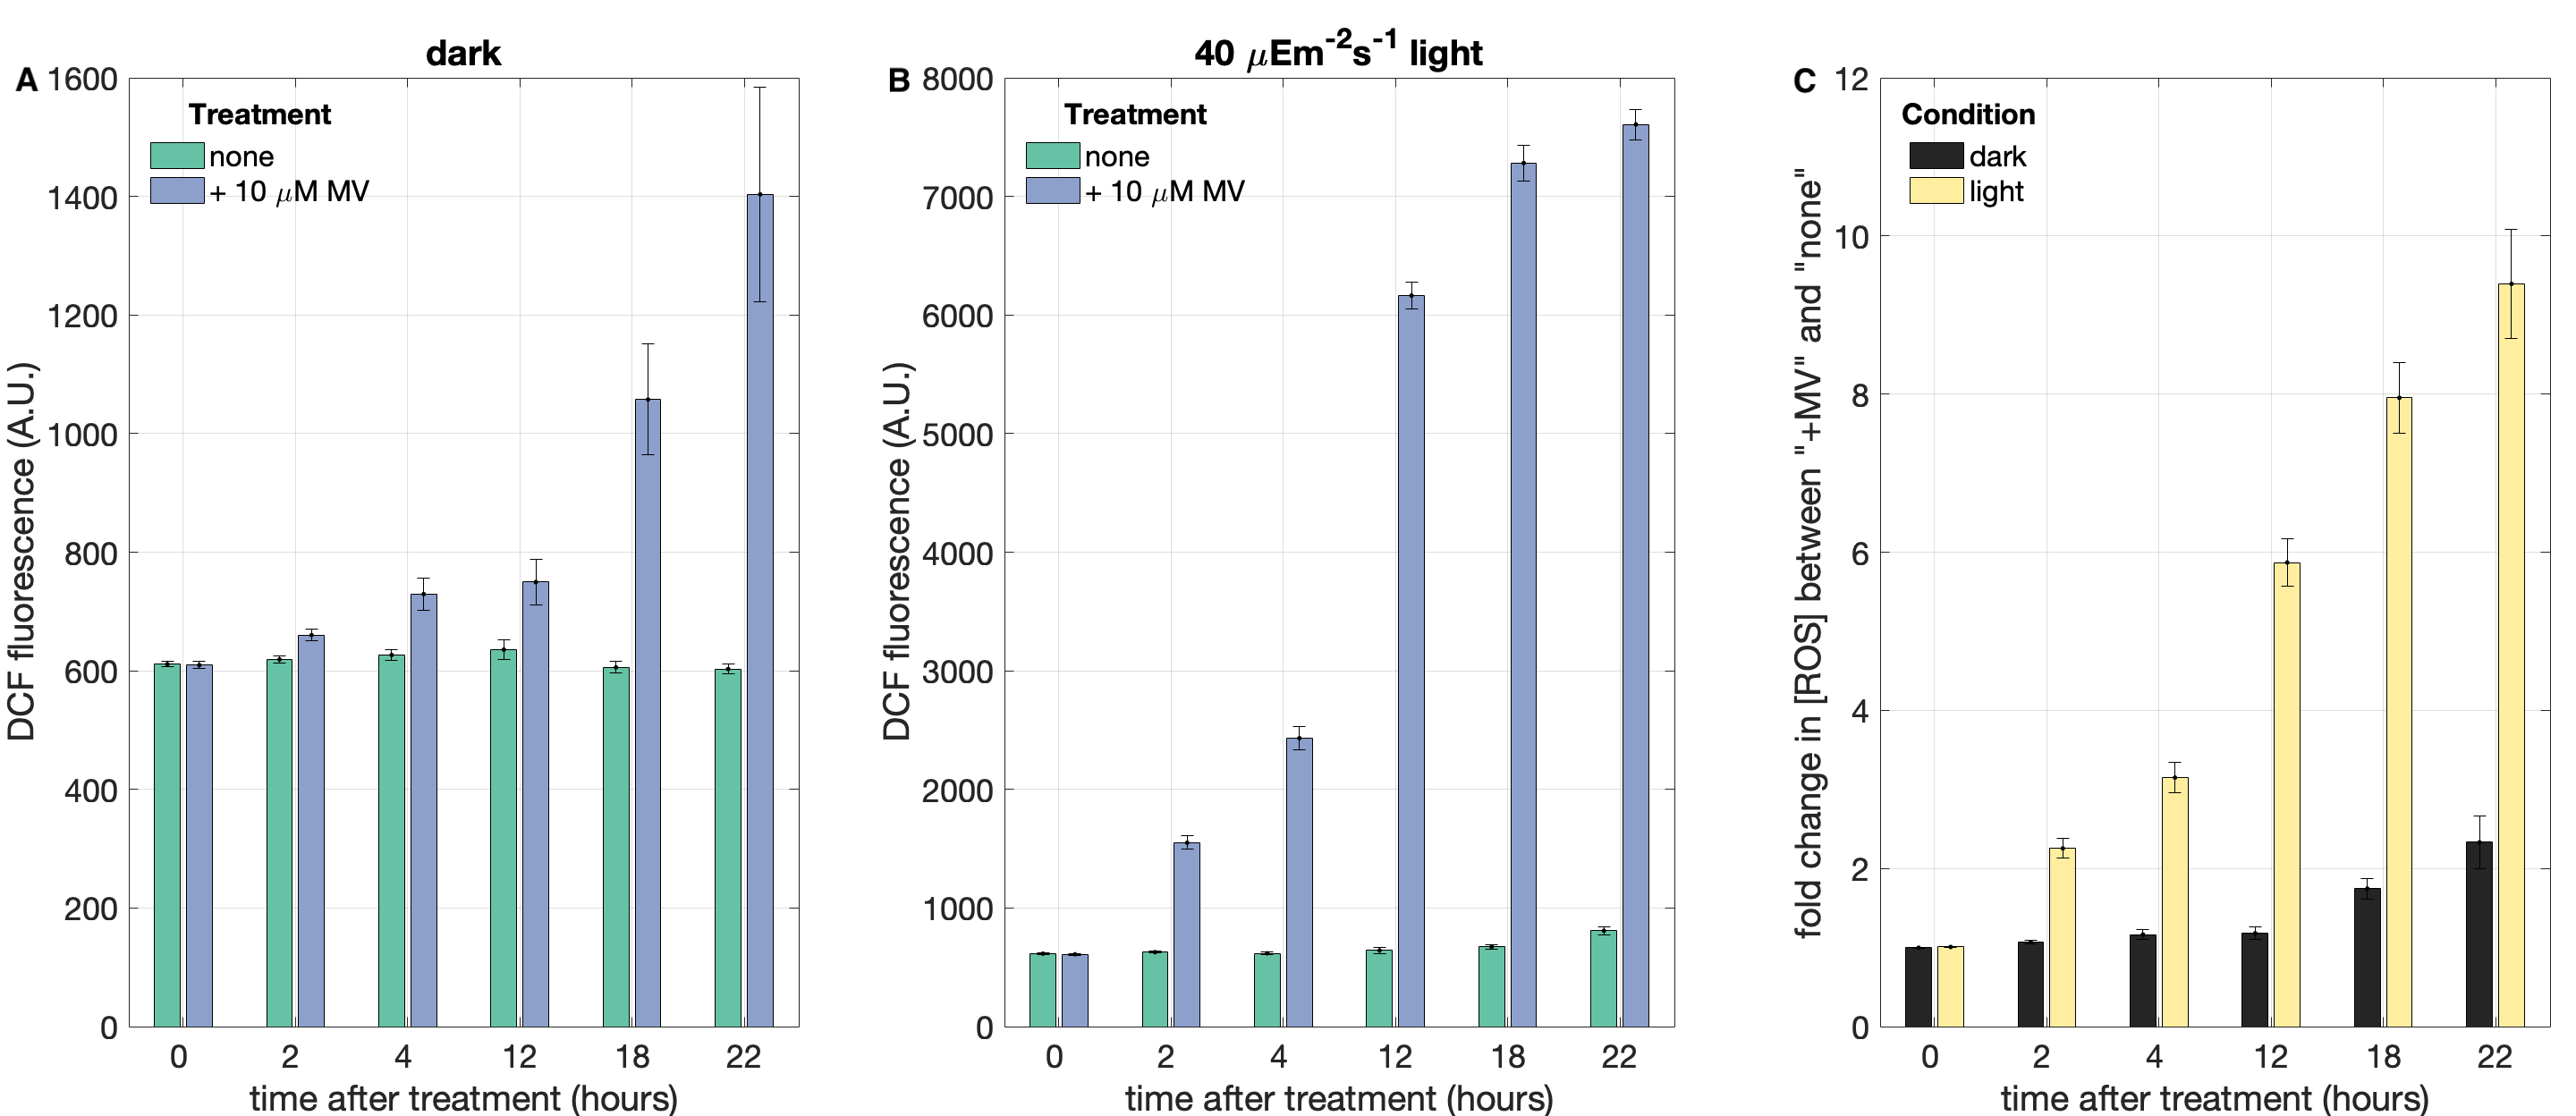
\includegraphics[width=\hsize]{../Figures/MV_adaptation/MV_ROS_DFCDA_Syn6803.png}
    \caption{ROS quantification assay based on the substrate DCFH-DA, which becomes fluorescent upon reaction with intracellular reactive oxygen species. A) DCF fluorescence in cultures of \textit{Synechocystis} at various time points after treatment with 10 $\mu$M methyl viologen (in the dark). B) DCF fluorescence at various time points after treatment with 10 $\mu$M MV (under 40 $\mu$mol$\cdot$m$^{-2}\cdot$s$^{-1}$ of white light illumination). C) Fold changes in DCF fluorescence between cultures treated with methyl viologen and no treatment control in the darkness and light at various time points. Error bars represent standard error of the mean from three biological replicates (individual colonies treated independently).}
    \label{fig:spectraMV1}
\end{figure}

\section{Adaptation to methyl viologen is not due to its abiotic degration over time}

\begin{figure}[H]
    \centering
    
\includegraphics[width=\hsize]{../Figures/MV_adaptation/growth_curves_firstevolution_Wt_6umMV.png}
    \caption{Growth curves of three independent unadapted (A) and MV-adapted (B) cultures of \textit{Synechocystis sp.} PCC 6803 growing at 30$^\circ$C under constant illumination (intensity = 100 $\mu$mol$\cdot$m$^{-2}\cdot$s$^{-1}$) in the absence (green trace) and upon addition of 6 $\mu M$  methyl viologen (from a fresh stock) during exponential growth (purple trace). Shaded regions represent standard errors over the means from three biological replicates.}
    \label{fig:freshstock}
\end{figure}


\begin{figure}[H]
    \centering
    
\includegraphics[width=\hsize]{../Figures/MV_adaptation/spectra_endpoint_firstevolution_Wt_6umMV.png}
    \caption{Absorbance spectra of unadapted (A) and adapted (B) cultures of \textit{Synechocystis sp.} PCC 6803 after 6 days of growth at 30$^\circ$C under constant illumination (intensity = 100 $\mu$mol$\cdot$m$^{-2}\cdot$s$^{-1}$) in the absence (green trace) and upon addition  of 6 $\mu$M methyl viologen during mod-log phase (purple trace). Shaded regions represent standard errors over the means from three biological replicates.}
    \label{fig:spectraMV1}
\end{figure}

\section{Spot plates of strains grown in BG11 without or with MV (6 $\mu$M)}

\begin{figure}[H]
    \centering
    \includegraphics[width=\hsize]{../Figures/MV_adaptation/spotplates_MVadapted_sentforsequencing}
    \caption{Spot plates of 2 unadapted (first two columns on each plates) and 5 adapted (columns 3 to 7) cultures of \textit{Synechocystis sp.} PCC 6803 in BG11 plates without methyl viologen (A) and with the addition of 6 $\mu$M  methyl viologen (B). Rows correspond to consecutive 10-fold serial dilutions of culture inocula (all starting at on OD$_{750}$ = 1). Plates were grown at 30$^\circ$C under constant illumination (intensity = 100 $\mu$mol$\cdot$m$^{-2}\cdot$s$^{-1}$) for 10 days.}
    \label{fig:spotassayMV}
\end{figure}


\section{Addition of methyl viologen at various growth phases}

\begin{figure}[H]
    \centering
    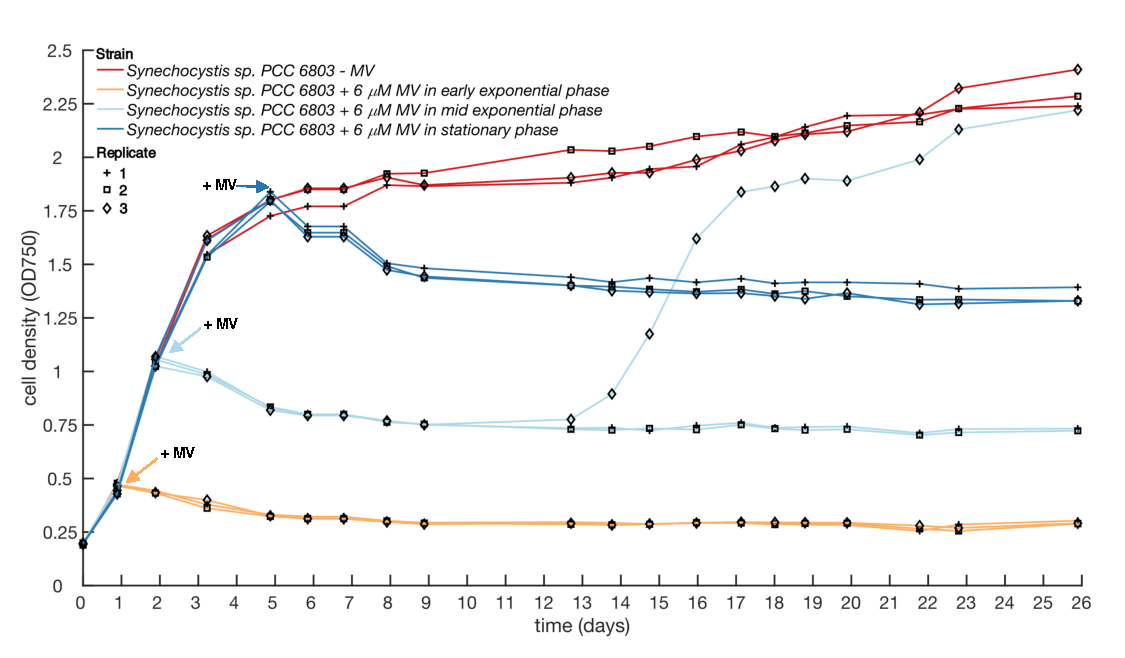
\includegraphics[width=\hsize]{../Figures/MV_adaptation/growthcurves_growthstages_Howe.pdf}
    \caption{Growth curves of \textit{Synechocystis sp.} PCC 6803 strains grown at 30 $^\circ$C under constant illumination (intensity = 40 $\mu$mol$\cdot$m$^{-2}\cdot$s$^{-1}$) in the absence (red trace) and upon addition  of 6 $\mu$M  methyl viologen during various growth stages (as indicated by the arrows colored according to the legend on top right).}
    \label{fig:MVgrowthstages}
\end{figure}


\section{The gene \textit{prqA} is not essential for spontaneous evolution of MV resistance}


\begin{figure}[H]
    \centering
    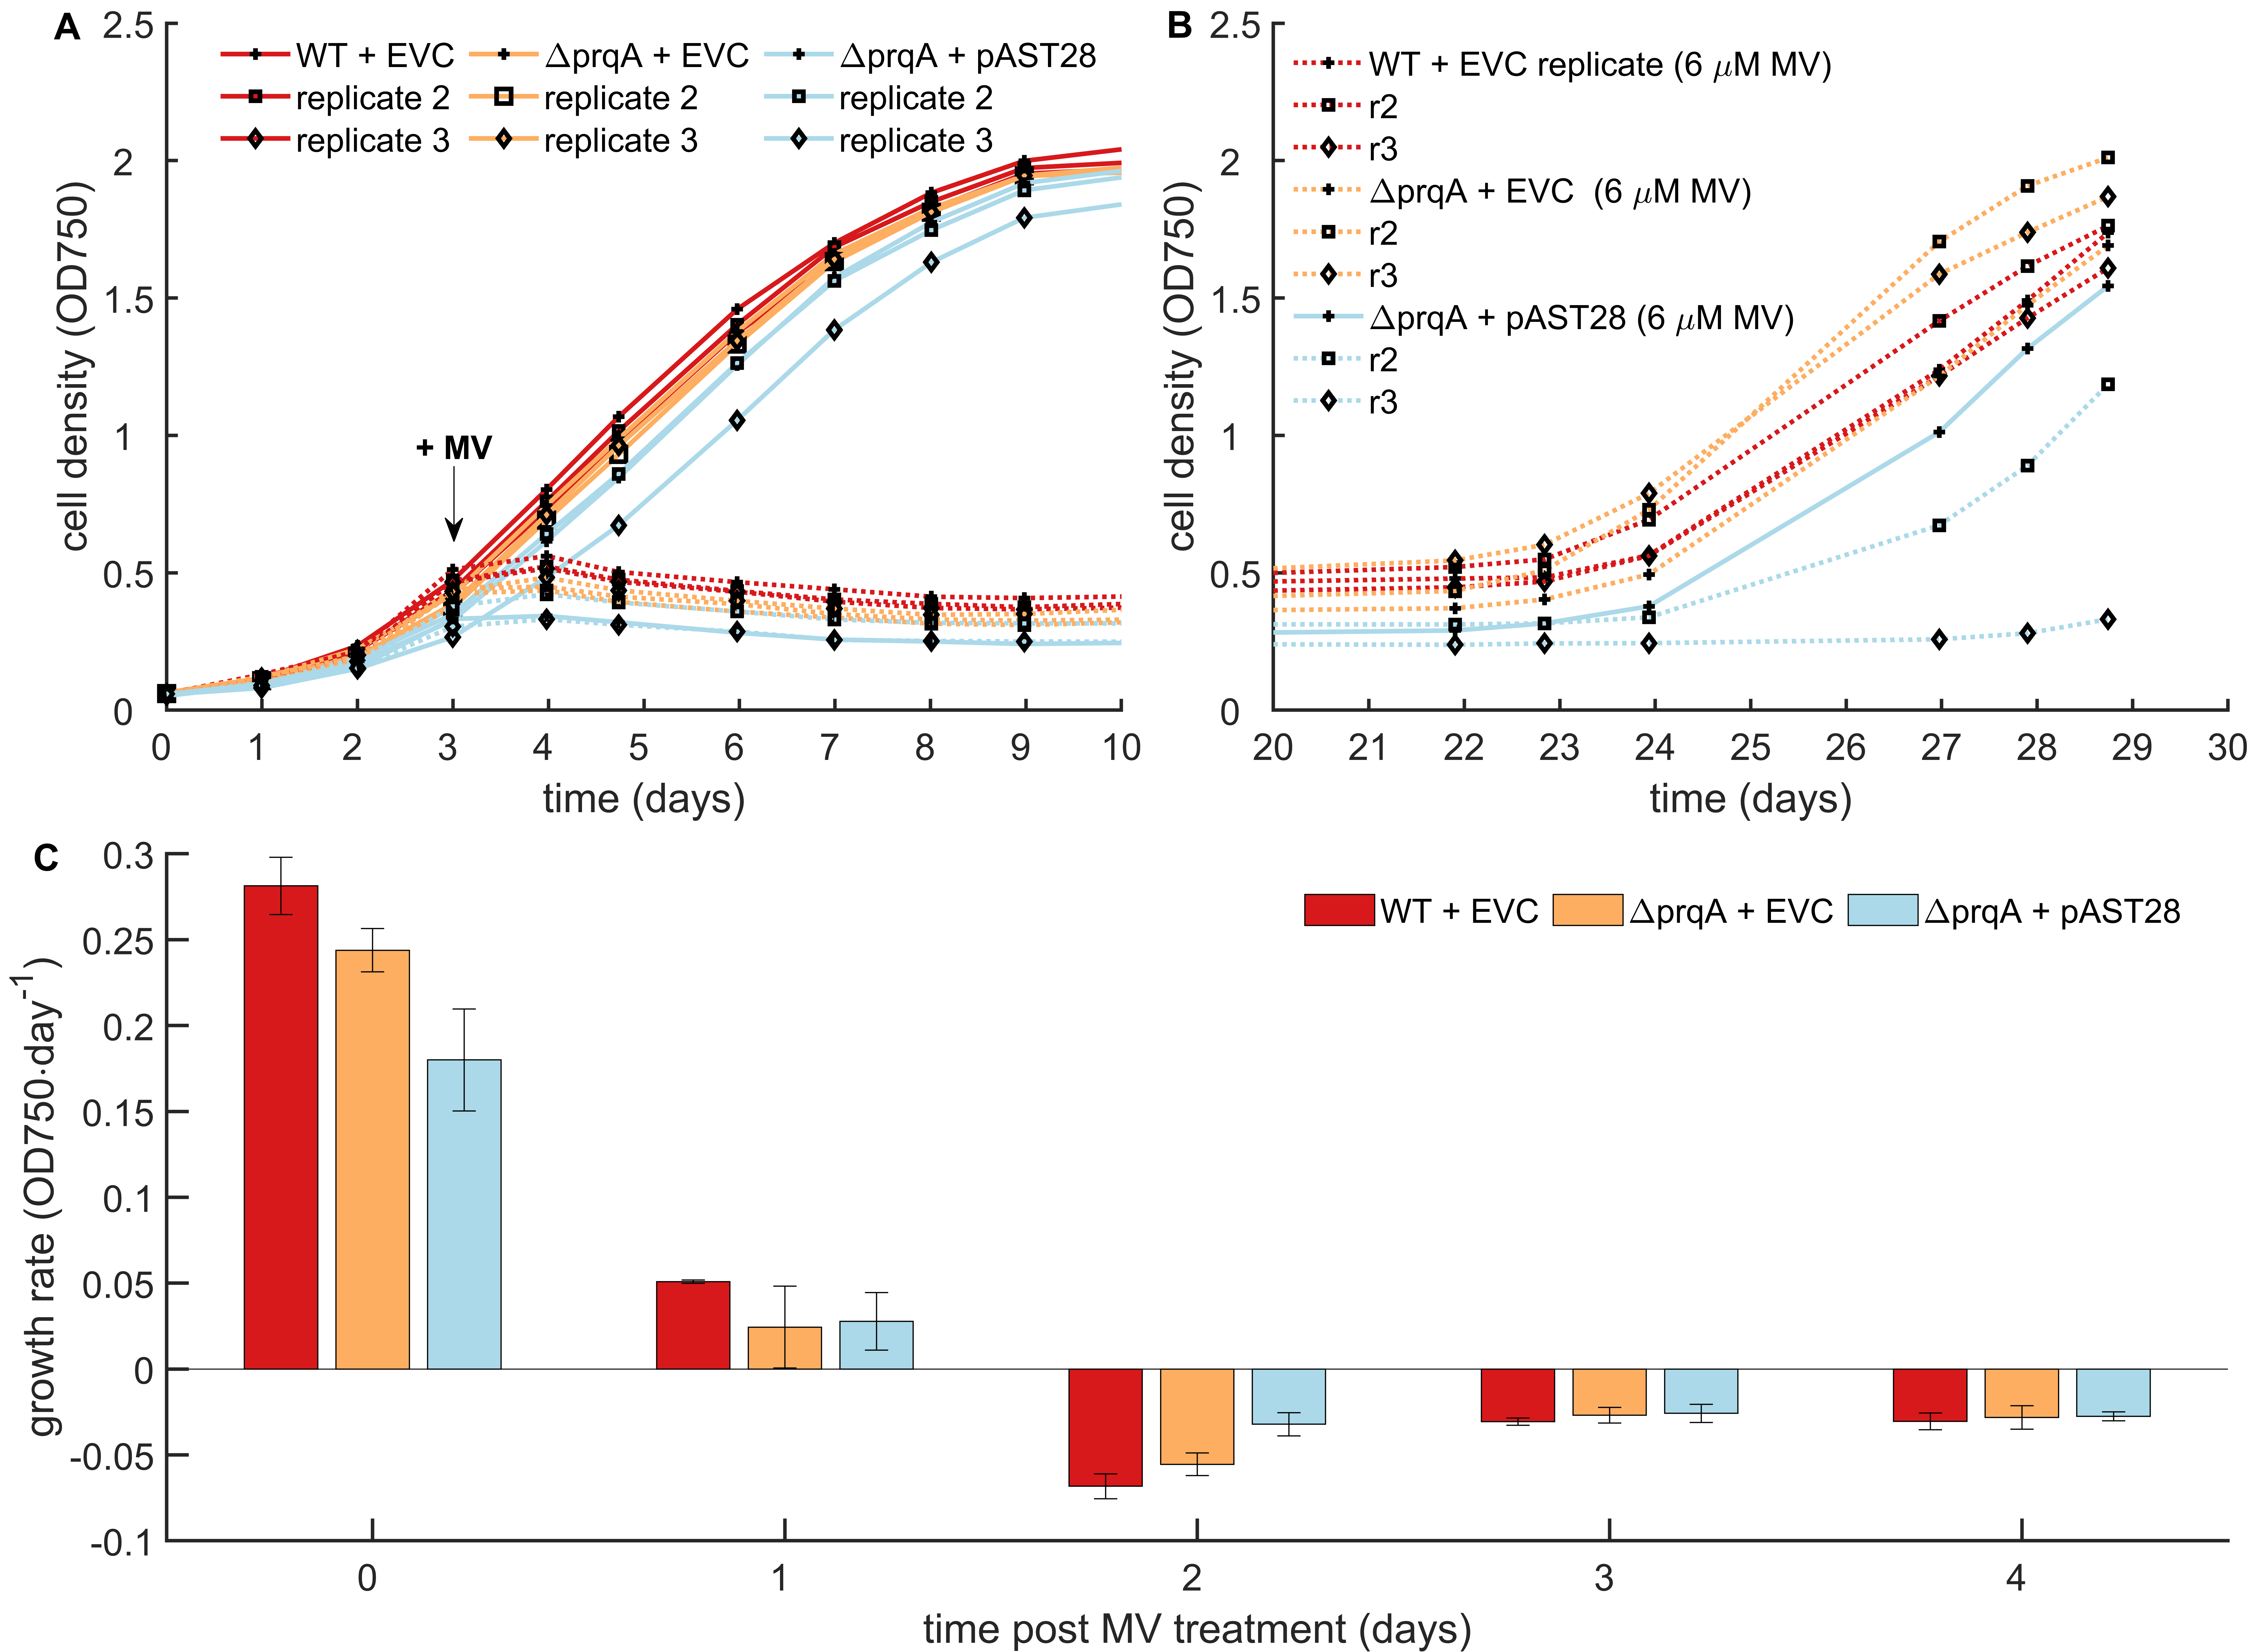
\includegraphics[width=\hsize]{../Figures/MV_adaptation/prqA_MvADapt_multipanel.png}
    \caption{Growth curves of wild-type, $\Delta$\textit{prqA} and complemented $\Delta$\textit{prqA} strains of \textit{Synechocystis sp.} PCC 6803 grown at 30 $^\circ$C under constant illumination (intensity = 100 $\mu$mol$\cdot$m$^{-2}\cdot$s$^{-1}$) in the absence (green trace) and upon addition  of 6 $\mu M$  methyl viologen during exponential growth (purple trace).}
    \label{fig:prqAMV}
\end{figure}


\section{Whole genome sequencing and bioinformatic analyses}


\subsection{Genome sequencing QC report}

\begin{table}[H]
    \centering
    \begin{tabular}{|c|c|c|c|c|c|c|c|}
    \hline
    \textbf{Sample} & \textbf{\begin{tabular}[c]{@{}c@{}}Concentration \\ (ng/$\mu$l)\end{tabular}} & \textbf{\begin{tabular}[c]{@{}c@{}}Volume \\ ($\mu$l)\end{tabular}} & \textbf{\begin{tabular}[c]{@{}c@{}}Effective \\ (\%)\end{tabular}} & \textbf{\begin{tabular}[c]{@{}c@{}}Error \\ (\%)\end{tabular}} & \textbf{\begin{tabular}[c]{@{}c@{}}Q20 \\ (\%)\end{tabular}} & \textbf{\begin{tabular}[c]{@{}c@{}}Q30 \\ (\%)\end{tabular}} & \textbf{\begin{tabular}[c]{@{}c@{}}GC \\ (\%)\end{tabular}} \\ \hline
    WT\_Nixon & 31.80 & 92 & 99.82 & 0.03 & 97.50 & 92.73 & 55.06 \\ \hline
    WT\_Howe & 27.80 & 98 & 99.78 & 0.03 & 96.75 & 90.99 & 46.50 \\ \hline
    mvR01\_Nixon & 36.40 & 95 & 99.77 & 0.03 & 97.43 & 92.60 & 52.66 \\ \hline
    mvR02\_Nixon & 25.00 & 97 & 99.78 & 0.03 & 97.34 & 92.30 & 47.98 \\ \hline
    mvR03\_Nixon & 30.00 & 101 & 99.81 & 0.03 & 97.65 & 93.02 & 48.64 \\ \hline
    mvR06\_Nixon & 44.60 & 98 & 99.80 & 0.03 & 97.19 & 91.96 & 51.59 \\ \hline
    mvR09\_Howe & 20.60 & 95 & 99.78 & 0.03 & 97.28 & 92.16 & 47.39 \\ \hline
    mvR10\_Howe & 20.20 & 95 & 99.86 & 0.03 & 97.66 & 93.39 & 47.83 \\ \hline
    mvR11\_Howe & 27.80 & 92 & 99.87 & 0.03 & 97.55 & 93.14 & 46.53 \\ \hline
    mvR12\_Howe & 19.60 & 98 & 99.86 & 0.03 & 97.65 & 93.31 & 47.50 \\ \hline
    \end{tabular}
\end{table}

Alignment of the trimmed and paired reads from whole genome sequencing experiments was carried out against several reference genome sequences of \textit{Synechocystis} substrains (Figures \ref{fig:WTN_NC000911} and \ref{fig:WTN_NC000911}). \ref{fig:SNPs} shows the results of the type and number of mutations of both wild types as compared to all \textit{Synechocystis} substrain reference genomes available in the NCBI datatase. For both wild-types, the GT-Kazusa reference genome was the one that resulted in the least amount of SNPs.

\begin{figure}[H]
    \centering
    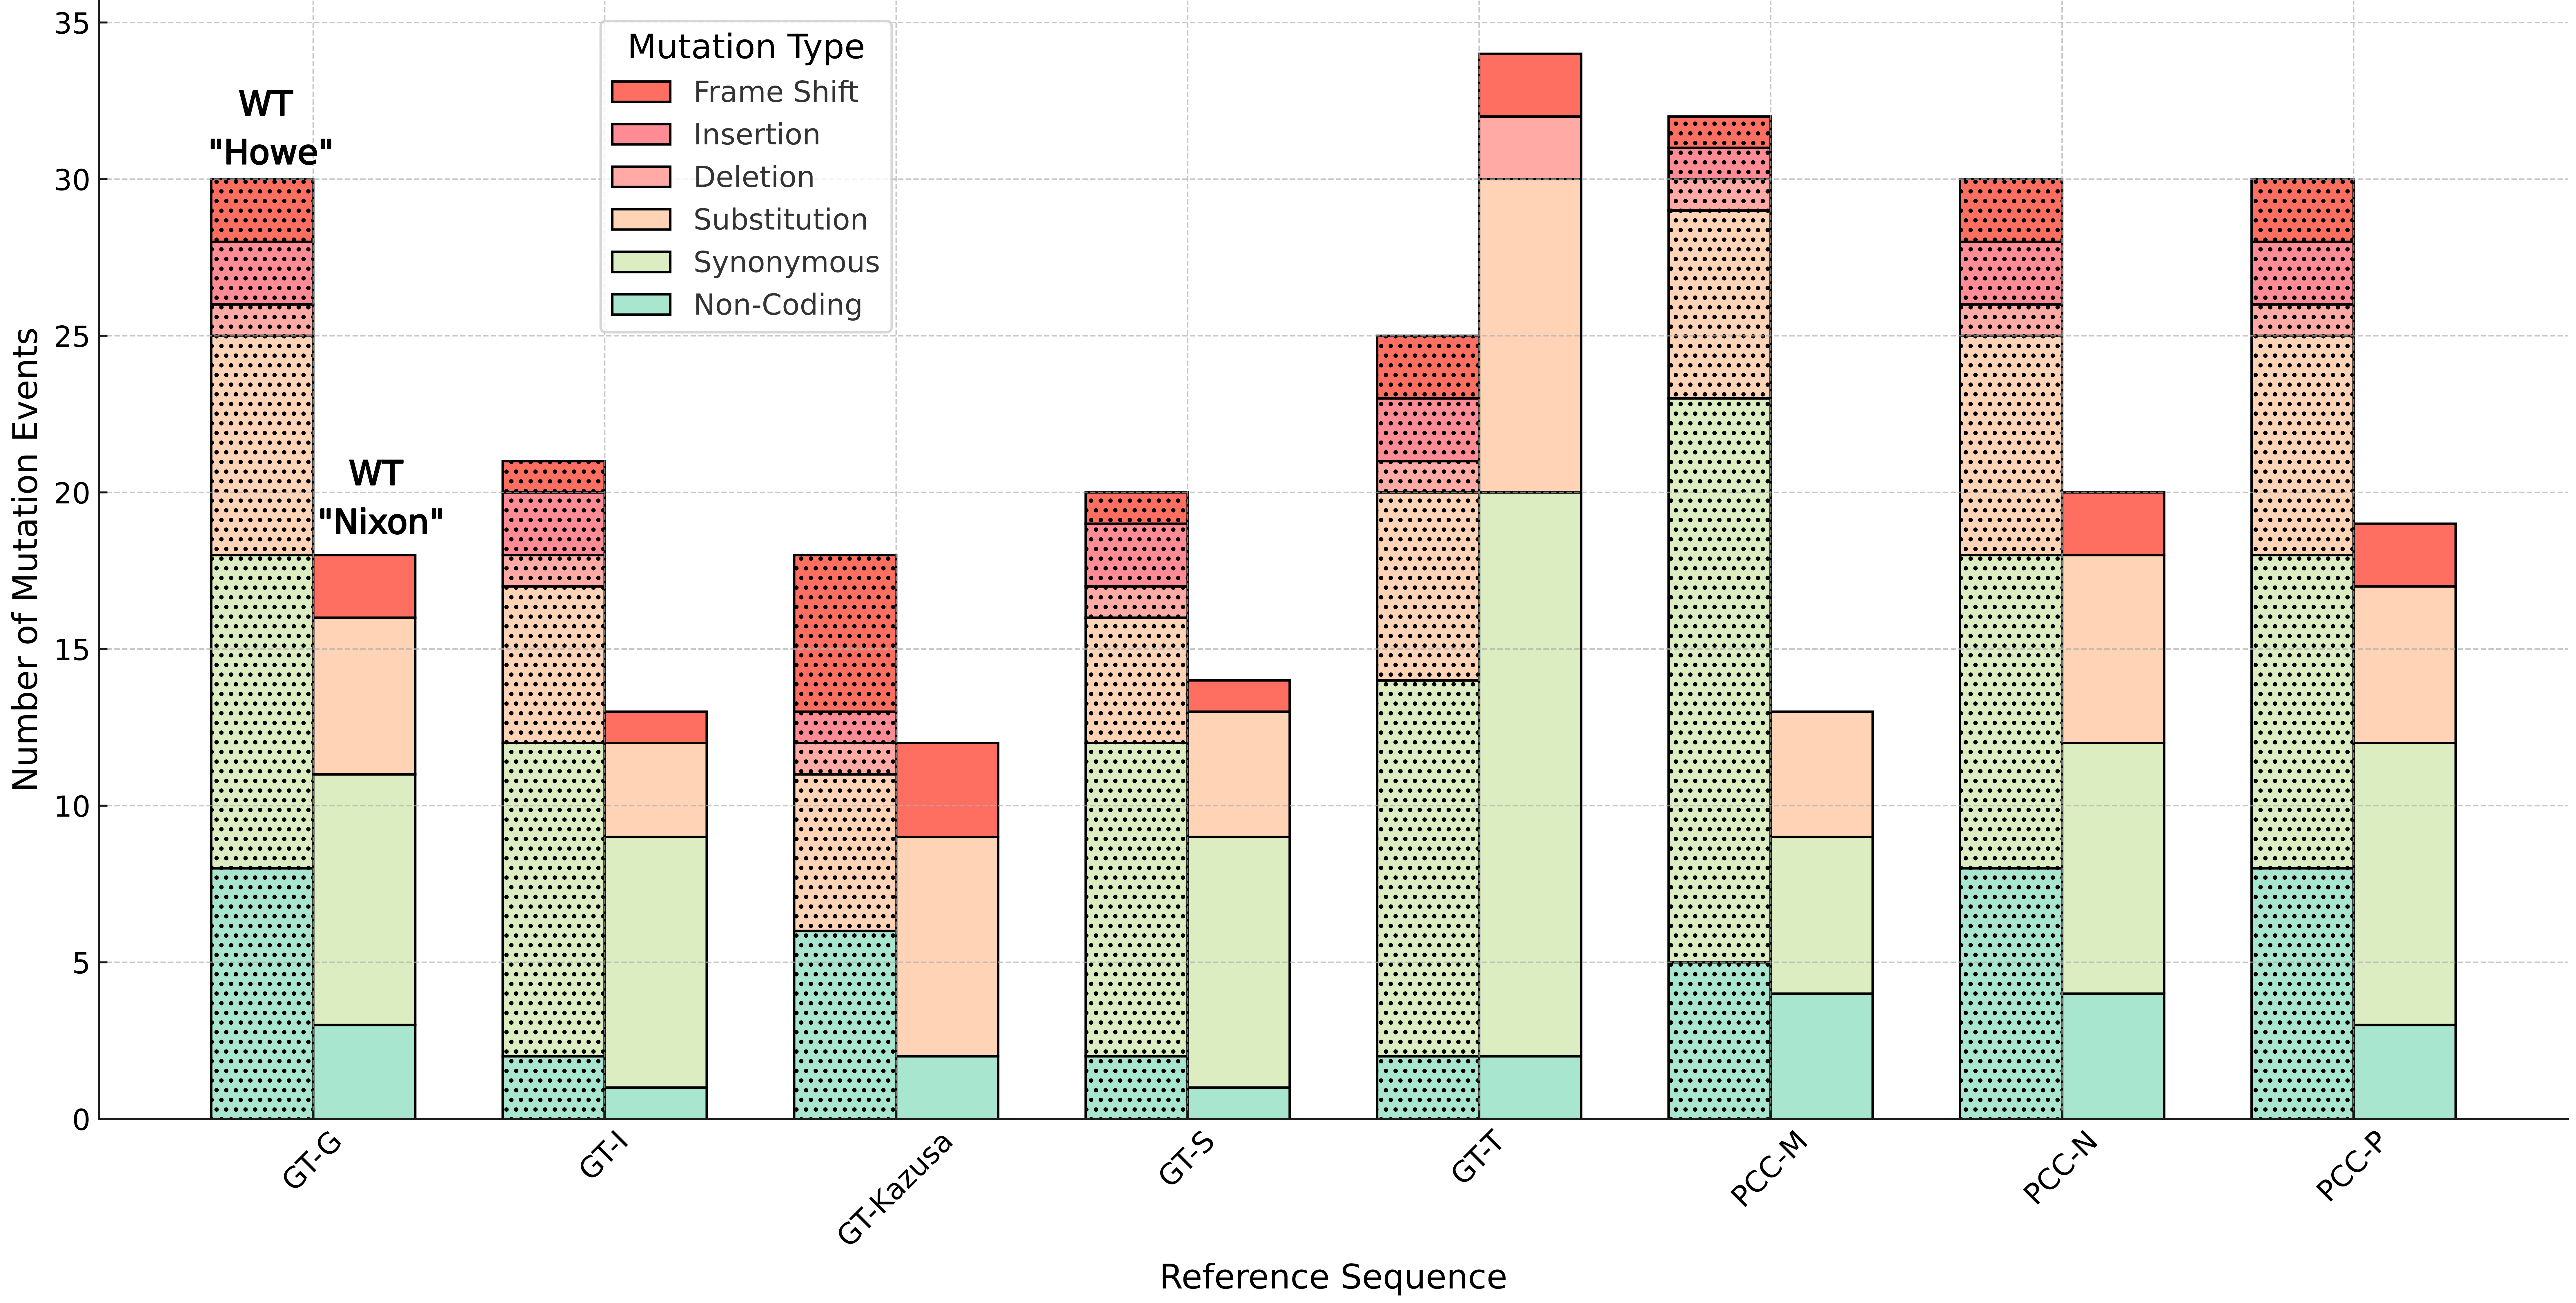
\includegraphics[width=\hsize]{../Figures/MV_adaptation/mutation_events_plot.png}
    \caption{Overview of the variant analysis results.}
    \label{fig:SNPs}
\end{figure}

The mutations were then filtered to identify only non-synonymous ones which results in mutated proteins. 

\begin{figure}[H]
    \centering
    \includegraphics[width=\hsize]{../Figures/WGS/wt_Nixon_vs_NC000911_genomeview.png}
    \caption{Trimmed and paired reads from whole genome sequencing experiments of \textit{Synechocystis} "Nixon'' wild-type aligned to the reference GT-"Kazusa'' strain (NC000911). Numbered are mutation events found within coding sequences of the reference genome.}
    \label{fig:WTN_NC000911}
\end{figure}

\begin{figure}[H]
    \centering
    \includegraphics[width=\hsize]{../Figures/WGS/wt_Howe_vs_NC000911_genomeview.png}
    \caption{Trimmed and paired reads from whole genome sequencing experiments of \textit{Synechocystis} "Howe'' wild-type aligned to reference "Kazusa'' strain (NC000911). Numbered are mutation events found within coding sequences of the reference genome.}
    \label{fig:WTH_NC000911}
\end{figure}

    \begin{table}[H]
        \centering
        \tiny	
        \begin{tabular}{c|c|c|c|c|c|c|c|c|}
        \cline{2-9}
        & \textbf{Gene} & \textbf{Product} & \begin{tabular}[c]{@{}c@{}}\textbf{CDS} \\ \textbf{Position}\end{tabular} & \textbf{Change} & \begin{tabular}[c]{@{}c@{}}\textbf{Protein} \\ \textbf{Effect}\end{tabular} & \begin{tabular}[c]{@{}c@{}}\textbf{Amino} \\ \textbf{Acid Change}\end{tabular} & \begin{tabular}[c]{@{}c@{}}\textbf{Variant} \\ \textbf{Frequency}\end{tabular} & \textbf{Reference} \\ \hline
        \multicolumn{1}{|c|}{1} & sll0020 & \begin{tabular}[c]{@{}c@{}}ATP-dependent  Clp protease \\ ATP-binding subunit\end{tabular} & 580 & T   -> G & Substitution & K   -> Q & 0.997 & GT-T \\ \hline
        \multicolumn{1}{|c|}{2} & sll0401 & citrate synthase & 434 & A -> C & Substitution & M -> R & 1 & PCC-M \\ \hline
        \multicolumn{1}{|c|}{3} & sll0414 & DUF4335   domain-containing protein & 334 & +C & Frame   Shift &  & 0.955 & GT-Kazusa \\ \hline
        \multicolumn{1}{|c|}{4} & sll0761 & hypothetical protein & 302 & -C & Frame Shift &  & 0.952 & GT-Kazusa \\ \hline
        \multicolumn{1}{|c|}{5} & sll0762 & Ig-like   domain-containing protein & 8924 & +C & Frame   Shift &  & 0.957 & GT-Kazusa \\ \hline
        \multicolumn{1}{|c|}{6} & sll0771 & sugar porter family MFS transporter & 85 & (C)8 -> (C)7 & Frame Shift &  & 0.919 & GT-T \\ \hline
        \multicolumn{1}{|c|}{7} & sll0789 & \begin{tabular}[c]{@{}c@{}}two-component   \\ system regulator RppA\end{tabular} & 403 & CCA   -> TCG & Substitution & W   -> R & \begin{tabular}[c]{@{}c@{}}0.517   \\ +- 0.003\end{tabular} & \begin{tabular}[c]{@{}c@{}}GT-Kazusa,  GT-I, GT-S, \\ GT-T, PCC-N, PCC-P, GT-G\end{tabular} \\ \hline
        \multicolumn{1}{|c|}{8} & sll0789 & \begin{tabular}[c]{@{}c@{}}two-component \\ system regulator RppA\end{tabular} & 397 & TTG -> GTC & Substitution & Q -> D & \begin{tabular}[c]{@{}c@{}}0.550\\  +- 0.0005\end{tabular} & \begin{tabular}[c]{@{}c@{}}GT-Kazusa, PCC-P, PCC-N, \\ GT-T, GT-S, GT-I, GT-G\end{tabular} \\ \hline
        \multicolumn{1}{|c|}{9} & sll0798 & sensor   histidine kinase RppB & 1339 & A   -> C & Substitution & F   -> V & 0.501 & PCC-M \\ \hline
        \multicolumn{1}{|c|}{10} & sll0798 & sensor histidine kinase RppB & 1336 & T -> G & Substitution & I -> L & 0.516 & PCC-M \\ \hline
        \multicolumn{1}{|c|}{11} & sll1201 & Rpn  family nuclease/putative transposase & 340 & C   -> A & Substitution & V   -> L & 0.509 & PCC-M \\ \hline
        \multicolumn{1}{|c|}{12} & sll1389 & hypothetical protein & 430 & (G)8 -> (G)7 & Frame Shift &  & \begin{tabular}[c]{@{}c@{}}0.89 +- \\ 0.012\end{tabular} & \begin{tabular}[c]{@{}c@{}}GT-Kazusa, PCC-P, PCC-N, \\ PCC-M, GT-T,  GT-S, GT-I, GT-G\end{tabular} \\ \hline
        \multicolumn{1}{|c|}{13} & sll1575 & serine/threonine-protein  kinase & 308 & +T & Frame   Shift &  & \begin{tabular}[c]{@{}c@{}}0.972   \\ +- 0\end{tabular} & PCC-N,  PCC-P \\ \hline
        \multicolumn{1}{|c|}{14} & sll1732 & \begin{tabular}[c]{@{}c@{}}NAD(P)H-quinone oxidoreductase \\ subunit F\end{tabular} & 1766 & C -> T & Substitution & R -> Q & 0.997 & GT-T \\ \hline
        \multicolumn{1}{|c|}{15} & sll1895 & EAL   domain-containing protein & 1134 & (T)3   -> (T)2 & Frame   Shift &  & 0.965 & GT-G \\ \hline
        \multicolumn{1}{|c|}{16} & sll1968 & anti-sigma regulatory factor & 124 & T -> C & Substitution & K -> E & 1 & GT-I \\ \hline
        \multicolumn{1}{|c|}{17} & slr0162 & type   II secretion system F protein & 420 & (G)9   -> (G)8 & Frame   Shift &  & 0.835 & GT-Kazusa \\ \hline
        \multicolumn{1}{|c|}{18} & slr0168 & DUF4114 domain-containing protein & 1207 & A -> G & Substitution & K -> E & 1 & GT-Kazusa \\ \hline
        \multicolumn{1}{|c|}{19} & slr0611 & solanesyl   diphosphate synthase & 205 & +ACGGCG & Insertion & -> TA & \begin{tabular}[c]{@{}c@{}}0.554   \\ +- 0\end{tabular} & \begin{tabular}[c]{@{}c@{}}GT-G,  GT-I, GT-S, \\ GT-T, PCC-N, PCC-P\end{tabular} \\ \hline
        \multicolumn{1}{|c|}{20} & slr0665 & bifunctional aconitate hydratase & 31 & G -> A & Substitution & D -> N & \begin{tabular}[c]{@{}c@{}}0.515 \\ +- 0\end{tabular} & \begin{tabular}[c]{@{}c@{}}GT-Kazusa, PCC-P, PCC-N, \\ GT-T, GT-S,  GT-I, GT-G\end{tabular} \\ \hline
        \multicolumn{1}{|c|}{21} & slr0665 & bifunctional   aconitate hydratase & 26 & T   -> C & Substitution & V   -> A & \begin{tabular}[c]{@{}c@{}}0.518   \\ +- 0\end{tabular} & \begin{tabular}[c]{@{}c@{}}GT-Kazusa,  PCC-P, PCC-N, \\ GT-T, GT-S, GT-I, GT-G\end{tabular} \\ \hline
        \multicolumn{1}{|c|}{22} & slr0667 & IS5 family transposase & 443 & +CATGGA & Insertion & G -> VHG & \begin{tabular}[c]{@{}c@{}}0.836 \\ +- 0.01\end{tabular} & \begin{tabular}[c]{@{}c@{}}GT-Kazusa, PCC-P, PCC-N, \\ PCC-M, GT-T,  GT-S, GT-I, GT-G\end{tabular} \\ \hline
        \multicolumn{1}{|c|}{23} & slr1085 & glycosyltransferase  family 4 protein & 67 & \begin{tabular}[c]{@{}c@{}}-GAACT\\ GTCCATC\end{tabular} & Deletion & ELSI   -> & \begin{tabular}[c]{@{}c@{}}0.74   \\ +- 0.043\end{tabular} & \begin{tabular}[c]{@{}c@{}}GT-Kazusa,  PCC-P, PCC-N, \\ PCC-M, GT-T, GT-S, GT-I, GT-G\end{tabular} \\ \hline
        \multicolumn{1}{|c|}{24} & slr2031 & \begin{tabular}[c]{@{}c@{}}PP2C family protein-serine/threonine \\ phosphatase\end{tabular} & 25 & A -> T & Substitution & S -> C & 1 +- 0 & GT-G, PCC-N, PCC-P \\ \hline
        \multicolumn{1}{|c|}{25} & slr2031 & \begin{tabular}[c]{@{}c@{}}PP2C family protein-serine/threonine \\ phosphatase\end{tabular} & 27 & CTT   -> AAA & Substitution & SL   -> RK & \begin{tabular}[c]{@{}c@{}}0.645   \\ +- 0.005\end{tabular} & GT-G \\ \hline
        \multicolumn{1}{|c|}{26} & slr2031 & \begin{tabular}[c]{@{}c@{}}PP2C family protein-serine/threonine  \\ phosphatase\end{tabular} & 42 & T -> A & Substitution & D -> E & \begin{tabular}[c]{@{}c@{}}0.6 \\ +- 0\end{tabular} & GT-G, PCC-N, PCC-P \\ \hline
        \multicolumn{1}{|c|}{27} & slr2122 & acylneuraminate cytidylyltransferase & 318 & C   -> G & Substitution & S   -> R & 1 & PCC-M \\ \hline
        \multicolumn{1}{|c|}{28} & ssl2749 & nucleotidyltransferase family protein & 74 & T -> C & Substitution & Q -> R & 0.534 & PCC-M \\ \hline
        \end{tabular}
        \label{Tab:NixMut}
        \caption{Unique mutations found in WT "Nixon''}
    \end{table}


    \begin{table}[H]
        \centering
        \tiny	
        \begin{tabular}{c|c|c|c|c|c|c|c|c|}
        \cline{2-9}
         & \textbf{Gene} & \textbf{Product} & \begin{tabular}[c]{@{}c@{}}\textbf{CDS} \\ \textbf{Position}\end{tabular} & \textbf{Change} & \begin{tabular}[c]{@{}c@{}}\textbf{Protein} \\ \textbf{Effect}\end{tabular} & \begin{tabular}[c]{@{}c@{}}\textbf{Amino Acid} \\ \textbf{Change}\end{tabular} & \begin{tabular}[c]{@{}c@{}}\textbf{Variant} \\ \textbf{Frequency}\end{tabular} & \textbf{Reference} \\ \hline
        \multicolumn{1}{|c|}{1} & sll0092 & transposase & 232 & A   -> G & Substitution & Y   -> H & \begin{tabular}[c]{@{}c@{}}0.557\\ +- 0\end{tabular} & \begin{tabular}[c]{@{}c@{}}GT-Kazusa, PCC-P, PCC-N, \\ GT-T, GT-S, GT-I, GT-G\end{tabular} \\ \hline
        \multicolumn{1}{|c|}{2} & sll0092 & transposase & 205 & G -> A & Substitution & P -> S & \begin{tabular}[c]{@{}c@{}}0.523 \\ +- 0\end{tabular} & GT-Kazusa, GT-G, GT-I \\ \hline
        \multicolumn{1}{|c|}{3} & sll0092 & transposase & 269 & T   -> C & Extension &  & \begin{tabular}[c]{@{}c@{}}0.614\\ +- 0\end{tabular} & \begin{tabular}[c]{@{}c@{}}GT-Kazusa, PCC-P, PCC-N, \\ GT-T, GT-S, GT-I, GT-G\end{tabular} \\ \hline
        \multicolumn{1}{|c|}{4} & sll0762 & hypothetical protein & 302 & -C & Frame Shift &  & 0.928 & GT-Kazusa \\ \hline
        \multicolumn{1}{|c|}{5} & sll1473 & PAS  domain S-box protein & 1397 & G   -> A & Substitution & A   -> V & 0.516 & GT-Kazusa \\ \hline
        \multicolumn{1}{|c|}{6} & sll1475 & ATP-binding protein & 15 & A -> T & Substitution & D -> E & 0.5 & GT-Kazusa \\ \hline
        \multicolumn{1}{|c|}{7} & sll1533 & \begin{tabular}[c]{@{}c@{}}type   IV pilus twitching motility \\ protein PilT\end{tabular} & 674 & -TGTTGA & Deletion & INK   -> K & 0.83 & GT-T \\ \hline
        \multicolumn{1}{|c|}{8} & sll1774 & \begin{tabular}[c]{@{}c@{}}Rpn family nuclease/putative \\ transposase\end{tabular} & 340 & TAA -> CAC & Substitution & L -> V & 0.552 & PCC-M \\ \hline
        \multicolumn{1}{|c|}{9} & slr0611 & solanesyl   diphosphate synthase & 205 & +CGGCG & Frame   Shift &  & \begin{tabular}[c]{@{}c@{}}0.503 \\ +- 0\end{tabular} & \begin{tabular}[c]{@{}c@{}}GT-G,  GT-I, GT-S, \\ GT-T, PCC-N, PCC-P\end{tabular} \\ \hline
        \multicolumn{1}{|c|}{10} & slr09240 & UPF0175 family protein & 200 & C -> A & Truncation &  & 0.508 & PCC-M \\ \hline
        \multicolumn{1}{|c|}{11} & slr1084 & hypothetical   protein & 230 & T   -> A & Substitution & V   -> D & \begin{tabular}[c]{@{}c@{}}0.547\\ +- 0\end{tabular} & \begin{tabular}[c]{@{}c@{}}GT-Kazusa,   \\ GT-S, GT-T\end{tabular} \\ \hline
        \multicolumn{1}{|c|}{12} & slr1274 & type IV pilus assembly protein PilM & 266 & T -> A & Substitution & V -> E & 1 & GT-T \\ \hline
        \multicolumn{1}{|c|}{13} & slr1510 & phosphate   acyltransferase PlsX & 263 & G   -> T & Substitution & G   -> V & 0.998 & PCC-N \\ \hline
        \multicolumn{1}{|c|}{14} & slr1609 & AMP-binding protein & 764 & T -> G & Substitution & F -> C & 1 +- 0 & \begin{tabular}[c]{@{}c@{}}GT-Kazusa, PCC-P, PCC-N, \\ GT-T, GT-S,   GT-I, GT-G\end{tabular} \\ \hline
        \multicolumn{1}{|c|}{15} & slr1712 & \begin{tabular}[c]{@{}c@{}}Rpn   family nuclease/putative \\ transposase\end{tabular} & 559 & CTG   -> ATT & Substitution & L   -> I & 0.611 & PCC-M \\ \hline
        \multicolumn{1}{|c|}{16} & slr1712 & \begin{tabular}[c]{@{}c@{}}Rpn family nuclease/putative \\ transposase\end{tabular} & 550 & G -> T & Substitution & A -> S & 0.641 & PCC-M \\ \hline
        \multicolumn{1}{|c|}{17} & slr1753 & CHAT   domain-containing protein & 3013 & A   -> C & Substitution & T   -> P & 0.521 & PCC-M \\ \hline
        \multicolumn{1}{|c|}{18} & slr1834 & photosystem I core protein PsaA & 1810 & G -> A & Substitution & V -> I & 0.994 & GT-Kazusa \\ \hline
        \multicolumn{1}{|c|}{19} & slr1862 & hypothetical   protein & 454 & +C & Frame   Shift &  & 0.538 & GT-Kazusa \\ \hline
        \multicolumn{1}{|c|}{20} & slr2031 & \begin{tabular}[c]{@{}c@{}}PP2C family protein-serine/threonine   \\ phosphatase\end{tabular} & 25 & AGC -> TGG & Substitution & S -> W & \begin{tabular}[c]{@{}c@{}}0.528 +- \\ 0.002\end{tabular} & GT-G, PCC-N, PCC-P \\ \hline
        \multicolumn{1}{|c|}{21} & slr2031 & \begin{tabular}[c]{@{}c@{}}PP2C   family protein-serine/threonine \\ phosphatase\end{tabular} & 29 & T   -> A & Truncation &  & \begin{tabular}[c]{@{}c@{}}0.543\\ +- 0\end{tabular} & GT-G,   PCC-N, PCC-P \\ \hline
        \multicolumn{1}{|c|}{22} & slr2031 & \begin{tabular}[c]{@{}c@{}}PP2C family protein-serine/threonine   \\ phosphatase\end{tabular} & 42 & T -> CGA & Frame Shift &  & \begin{tabular}[c]{@{}c@{}}0.51 \\ +- 0\end{tabular} & GT-G, PCC-N, PCC-P \\ \hline
        \multicolumn{1}{|c|}{23} & ssl0172 & transposase & 205 & G   -> A & Substitution & P -> S & \begin{tabular}[c]{@{}c@{}}0.523\\ +- 0\end{tabular} & GT-S, GT-T, PCC-N, PCC-P \\ \hline
        \end{tabular}
        \label{Tab:MutHowe}
        \caption{Unique mutations found in WT "Howe''}
    \end{table}




\subsection{Sequenced strains compared to various substrains}

To visualise the SNPs similarity between various strains, a principal component analysis (PCA)  was performed, where the feature matrix was constructed to represent each strain as a row and each reference genome as a column. The entries in this matrix were the total SNP counts for each strain against each reference genome. Thus, the PCA effectively reduced the multidimensional space spanned by the different reference genomes into a lower-dimensional representation. The PCA plot positions each strain based on its SNP profile across different reference genomes. Strains that are genomically similar in terms of SNP counts against multiple reference genomes would appear closer in the reduced-dimensional space.

\begin{figure}[H]
    \centering
    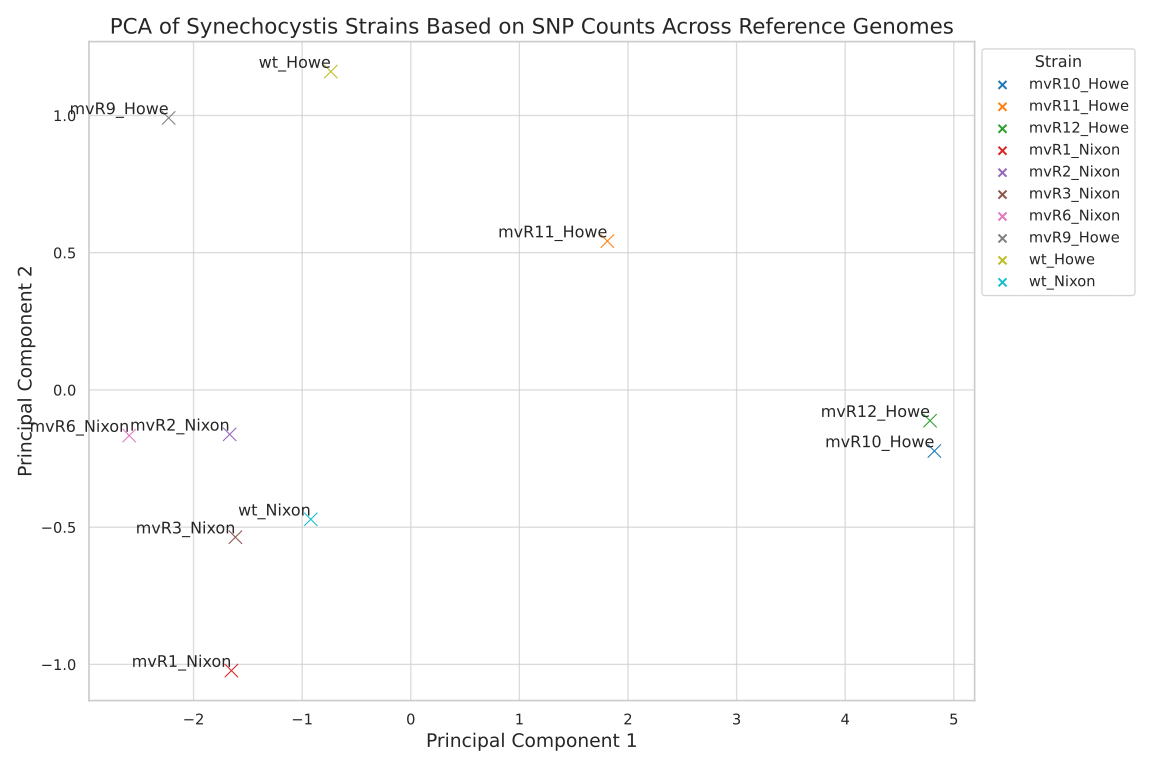
\includegraphics[width=\hsize]{../Figures/MV_adaptation/PCA_Synechocystis_Strains_SNP_Counts.png}
    \caption{Principal component analysis based on SNPs count of the sequenced genomes}
    \label{fig:PCA}
\end{figure}

Principal Component 1 (PC1) captured approximately 88.22\% of the total variance in the dataset. Principal Component 2 (PC2) accounted for about 5.37\% of the total variance. Cumulative Explained Variance: Together, the first two principal components capture approximately 93.58\% of the total variance. The first principal component (PC1) alone captures a significant proportion of the dataset's variance, indicating an effective reduction in dimensionality. The high cumulative explained variance (93.58\%) implies that the first two principal components provide a statistically robust representation of the dataset's original variability.
Therefore PCA analysis indicated that strains with the "Howe" and "Nixon" suffixes tend to cluster with their respective wild-types, corroborating the genomic closeness between mutants and their parental strains.

\subsection{SNPs Polimorphism}

\begin{figure}[H]
    \centering
    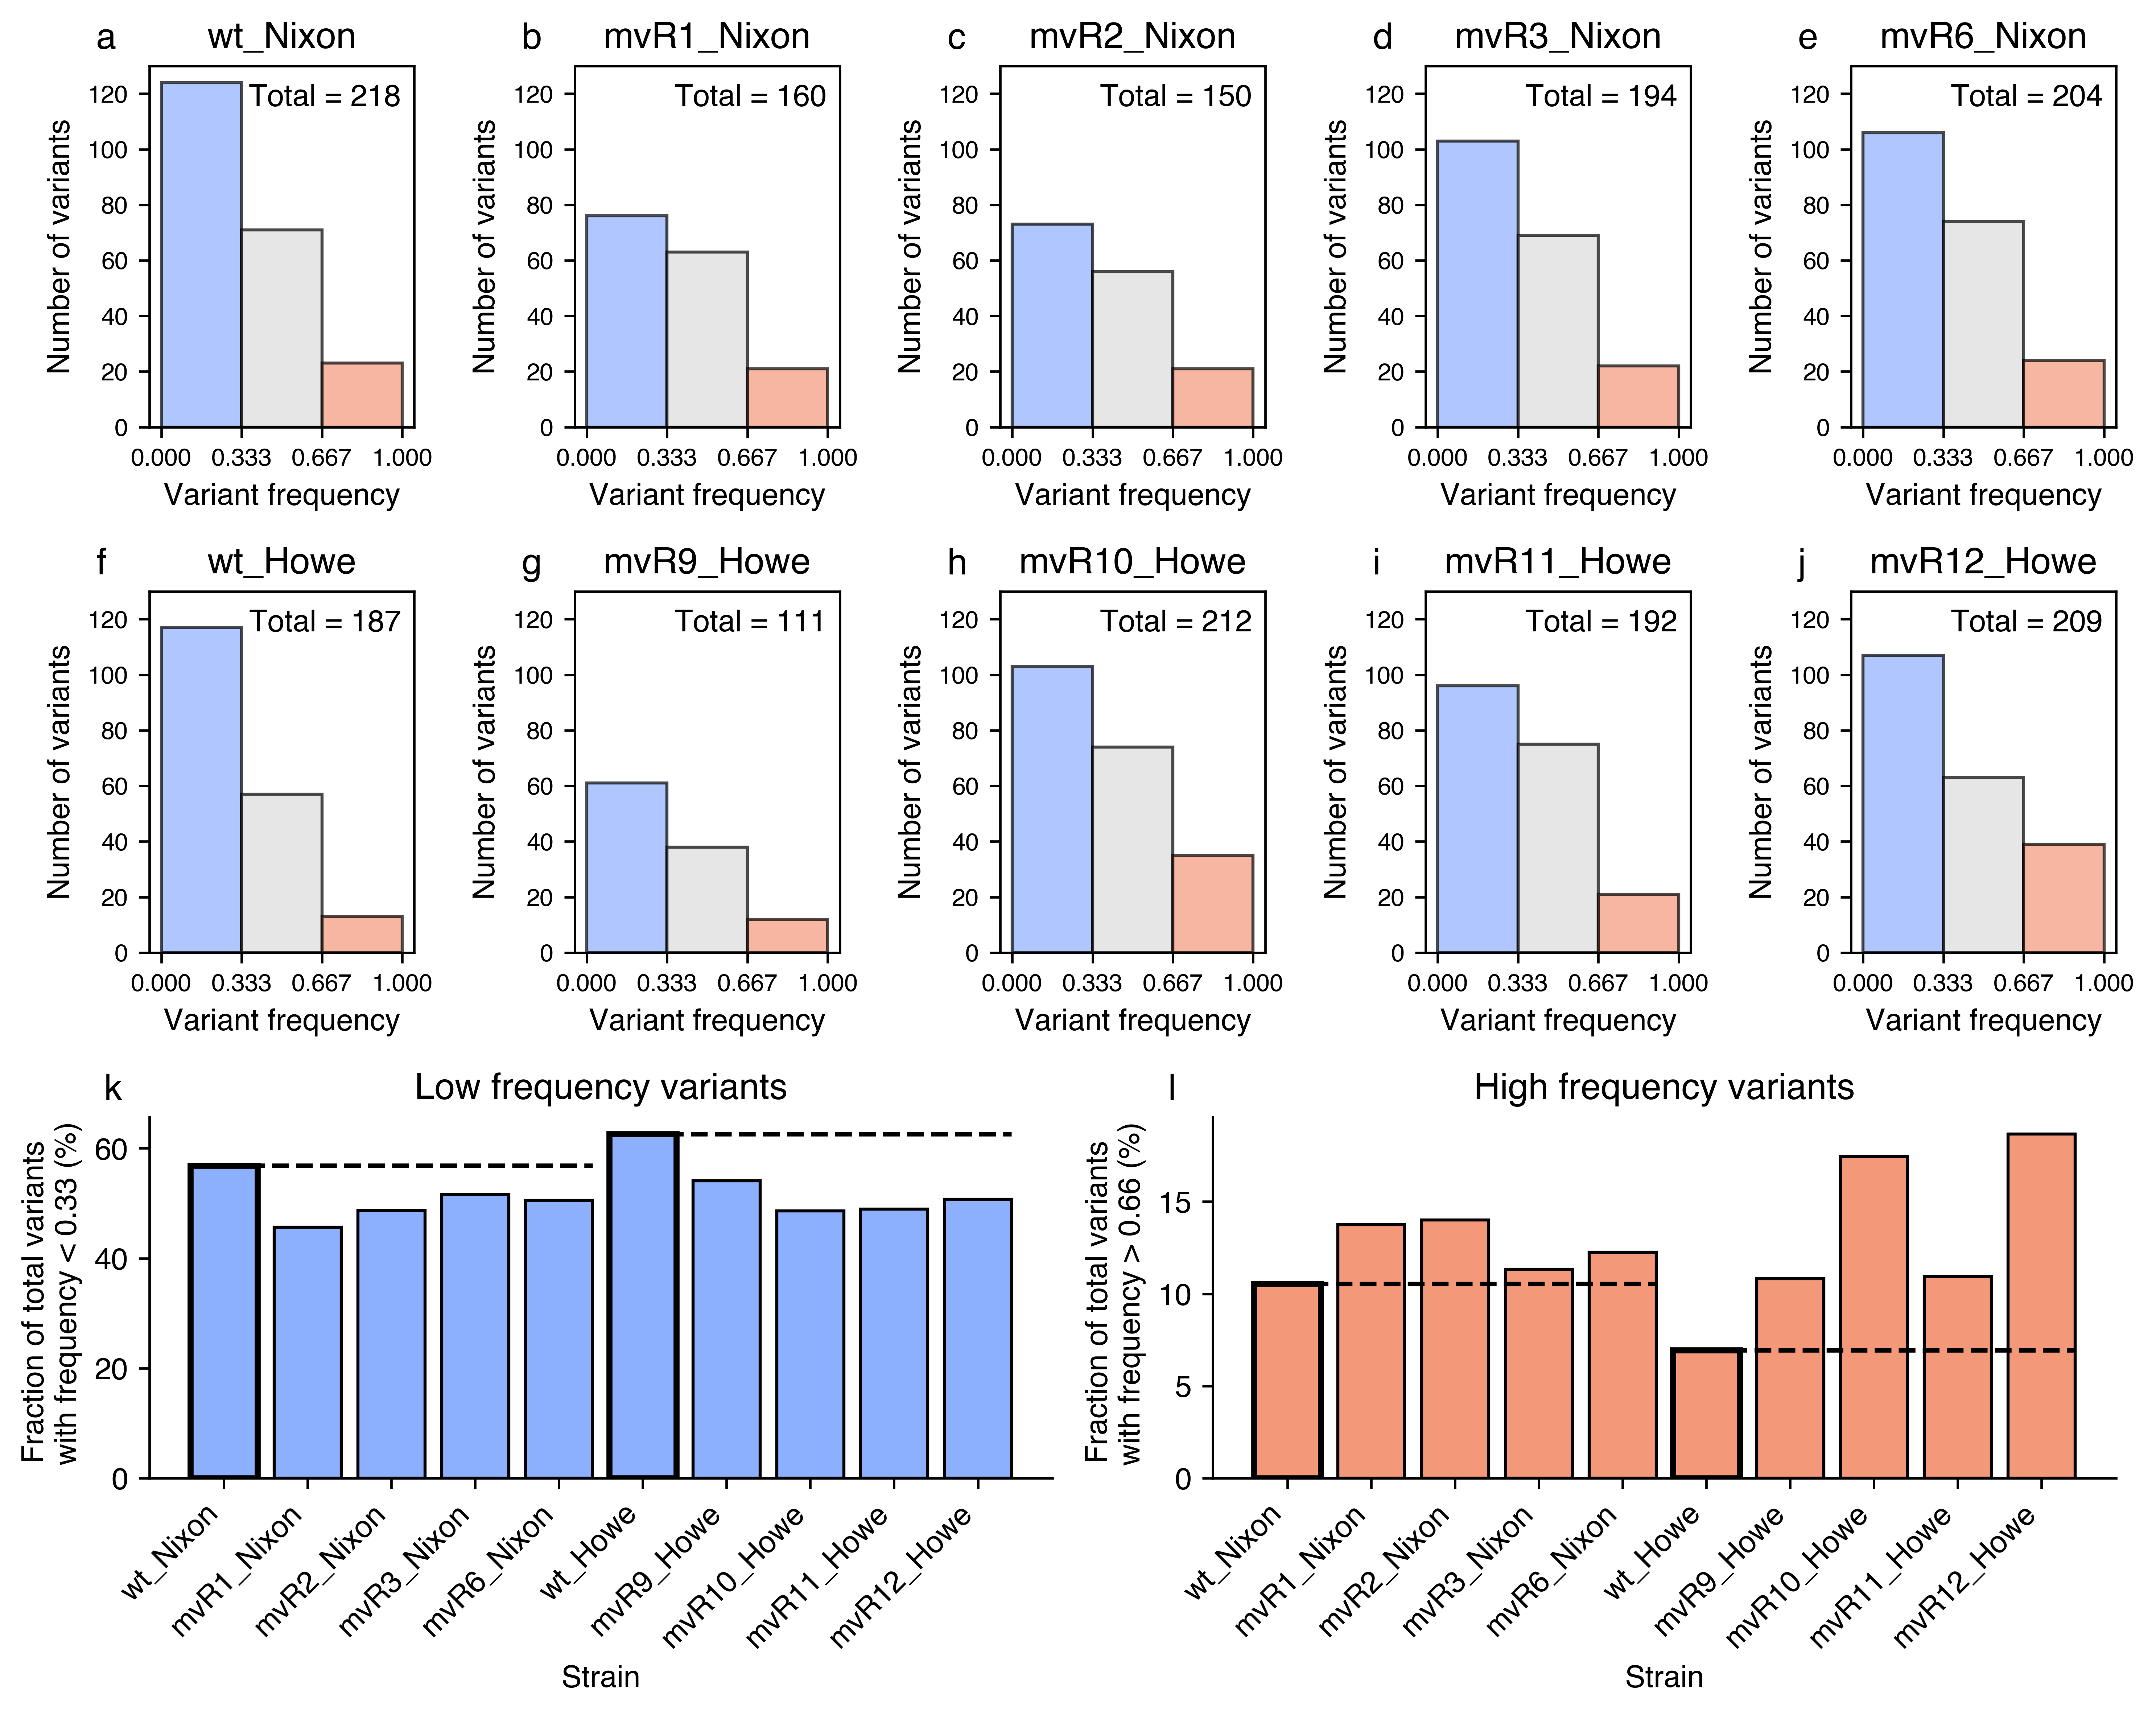
\includegraphics[width=\hsize]{../Figures/WGS/variant_frequency_fraction_comparison_3bins.png}
    \caption{3 bins, 0.3 and 0.6 as thresholds}
    \label{fig:3bins}
\end{figure}

\begin{figure}[H]
    \centering
    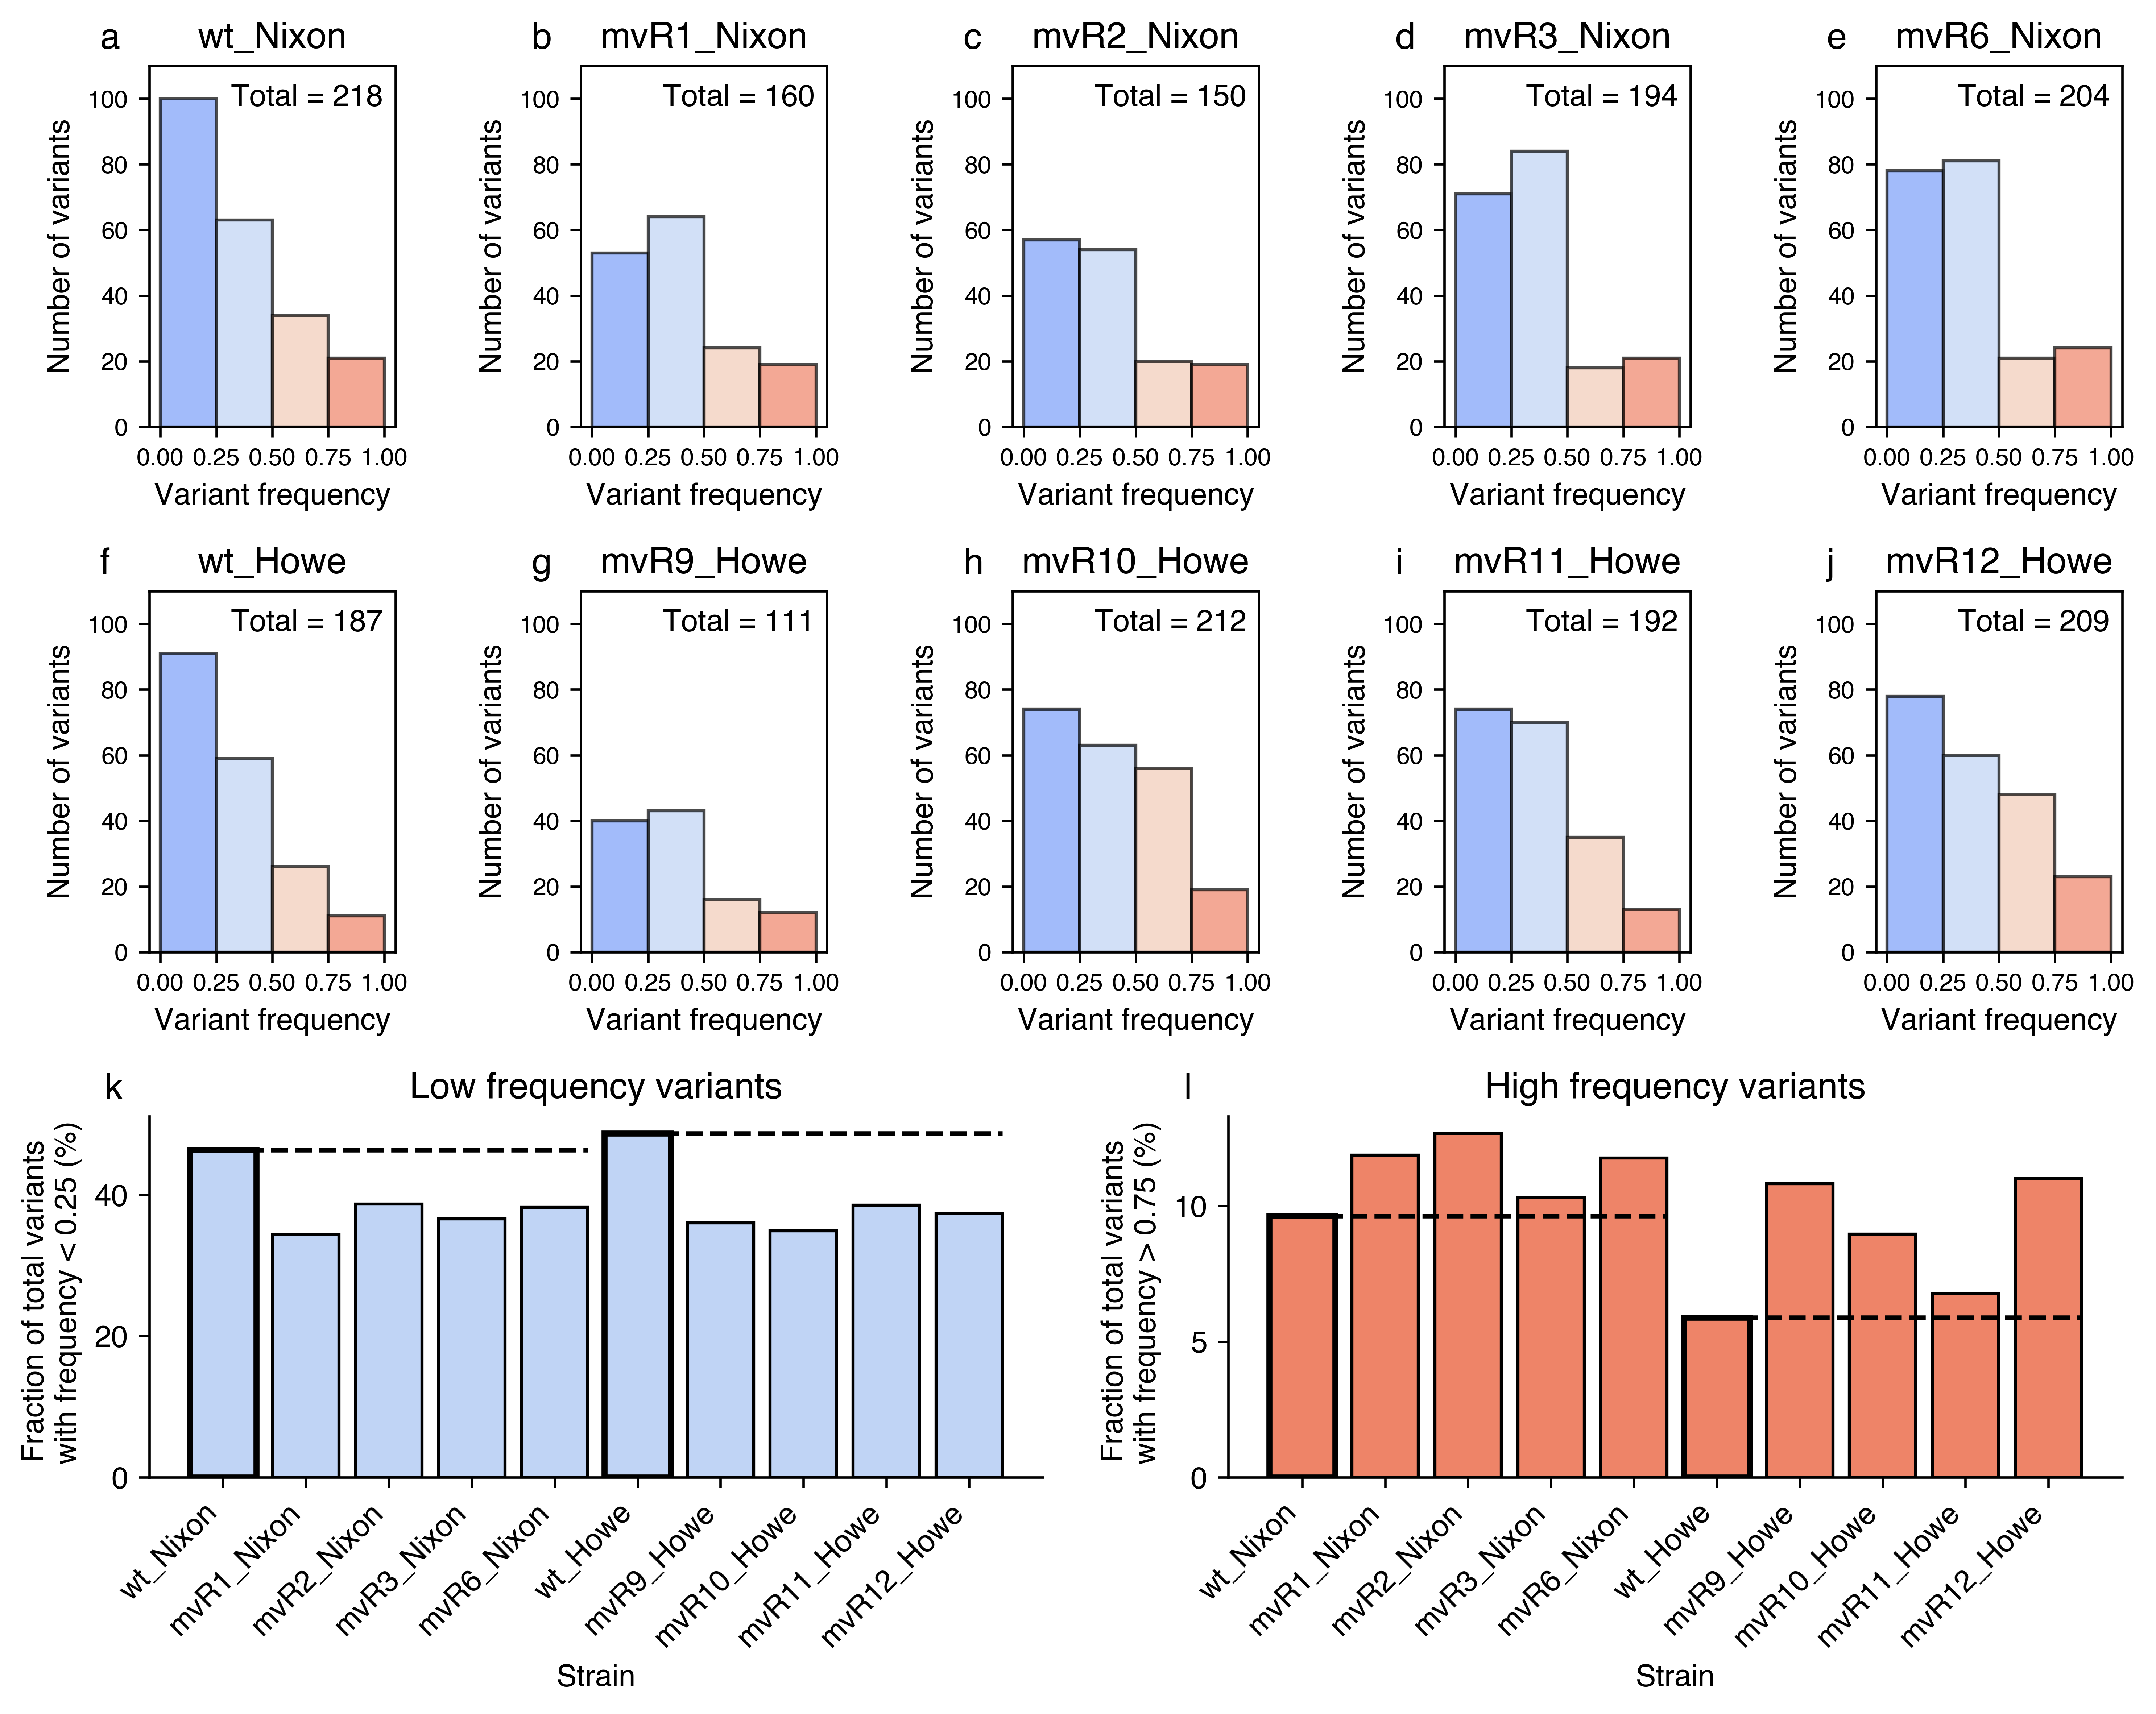
\includegraphics[width=\hsize]{../Figures/WGS/variant_frequency_fraction_comparison_4bins.png}
    \caption{4 bins, 0.25 and 0.75 as thresholds}
    \label{fig:4bins}
\end{figure}

\begin{figure}[H]
    \centering
    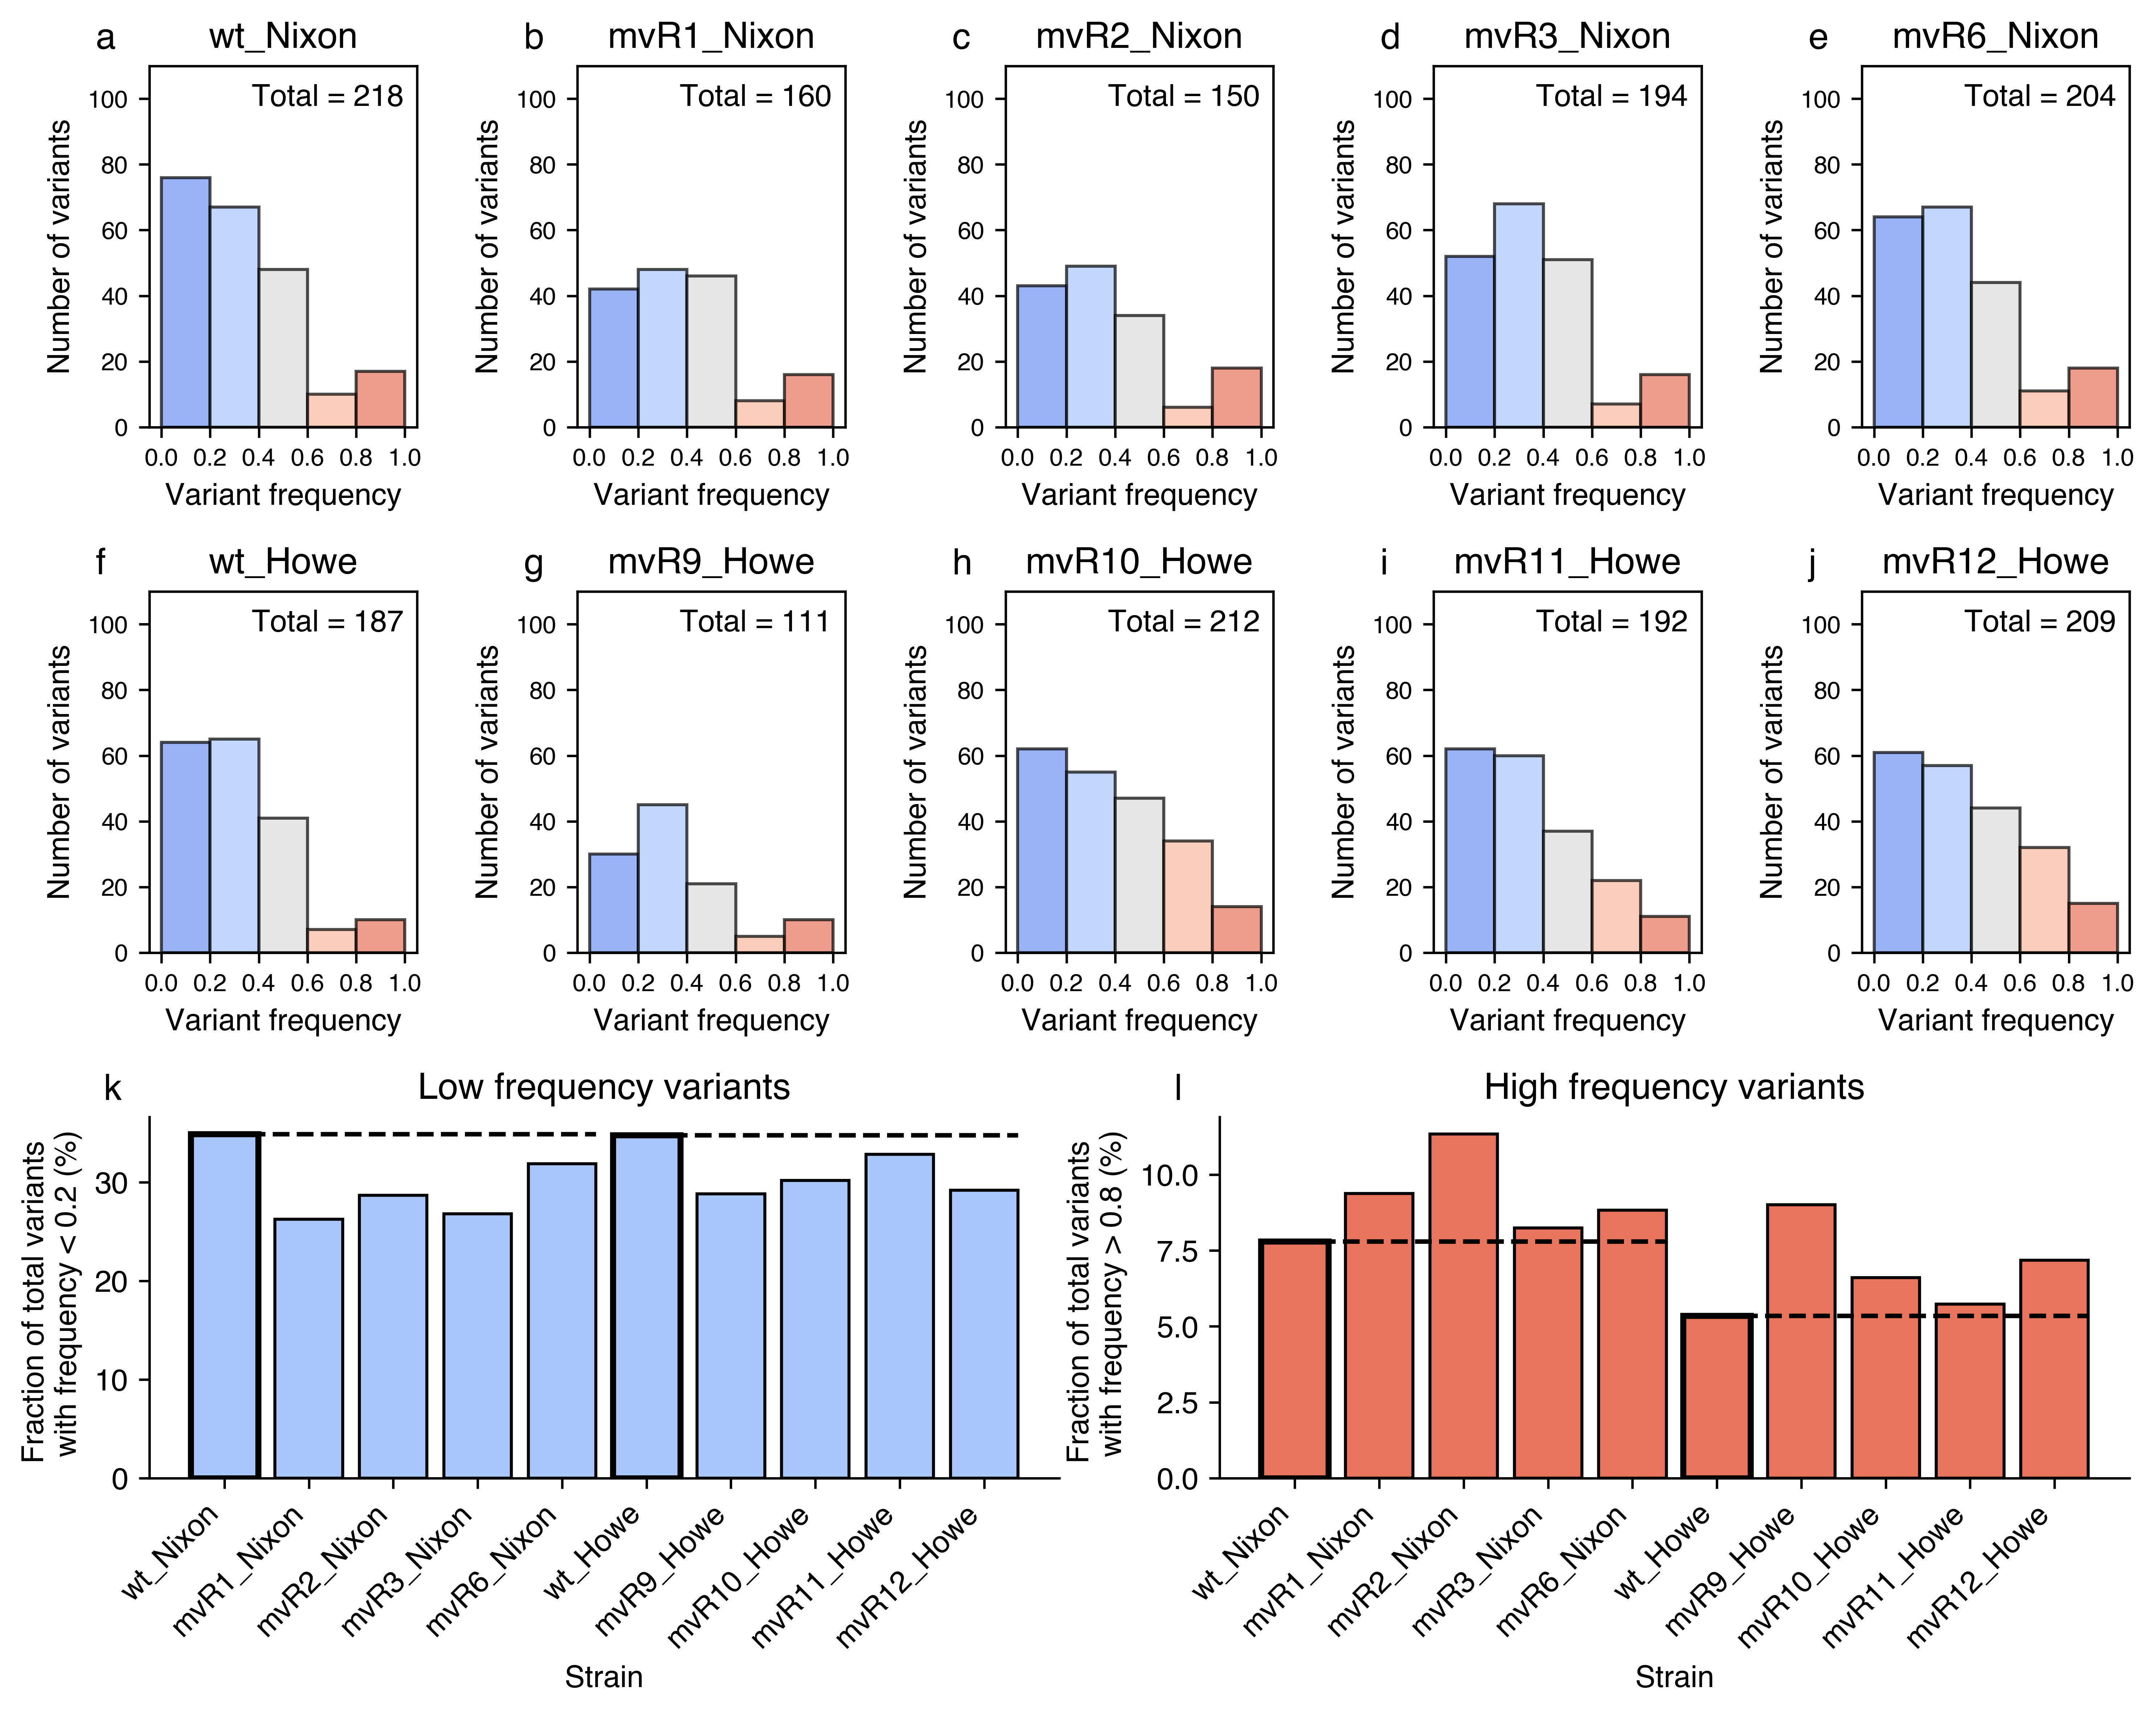
\includegraphics[width=\hsize]{../Figures/WGS/variant_frequency_fraction_comparison_5bins.png}
    \caption{5 bins, 0.2 and 0.8 as thresholds}
    \label{fig:5bins}
\end{figure}



\section{Extended methods}

\subsection{Buffers and media}

\subsubsection{0.25 M EDTA stock solution - pH8}
To prepare 100 ml of 0.25 M EDTA stock solution at pH = 8 (needed for preparing BG11):
\begin{enumerate}
	\item Weigh 9.305 g of Na$_2$EDTA (FW 372.2)
	\item Dissolve in $\approx$80 mL of DI water
	\item Adjust pH to 8 with concentrated NaOH
	\item Top up to final volume (100 mL) with deionised water
	\item Autoclave
\end{enumerate}


\subsubsection{1M Tris/HCl buffer - pH8}
To obtain 100 ml a 1M Tris/HCl buffer (required to prepare the pre-lysis buffer ``Smoker B’’ for gDNA extraction):
\begin{enumerate}
	\item Weigth 12.11 g of Tris
	\item Dissolve in $\approx$80 ml of deionised water
	\item Mix with magnetic stirrer until fully dissolved
	\item Adjust pH to 8 with concentrated HCl
	\item Top up to final volume (100 mL) with deionised water
	\item Autoclave
\end{enumerate} 

\subsubsection{Lysis buffer for gDNA extraction (``Smoker B’’)}\label{SBuffer}
Smoker B (SB) buffer was used in the pre-lysis step for genomic DNA extraction of cyanobacteria (tested for \textit{Synechocystis} and \textit{Chroococcidiopsis}). It contains lyophilised lysozyme powder from chicken egg whites for cell lysis, and RNAse and proteinase K to degrade unwanted RNA and protein materials, respectively. Lysozyme powder, RNAse and proteinase K were kept in the freezer (-20$^{\circ}$C). To prepare the buffer, the components listed in Table \ref{table:smokerB} were added in a 15 mL Falcon tube and vortex until fully dissolved. For genomic extraction, each sample requires 170 $\mu$l of Smoker B buffer. The solution was not autoclaved. Previously autoclaved water and stocks were used to prepare the solution fresh on the day of the experiment. 

\begin{table}[H]
    \centering
    \begin{tabular}{|c|c|c|c|}
    \hline
    \textbf{Ingredient} & \textbf{[Working]} & \textbf{[Stock]} & \textbf{\begin{tabular}[c]{@{}c@{}}Amount to add \\ (Final volume = 10 mL)\end{tabular}} \\ \hline
    \begin{tabular}[c]{@{}c@{}}1M Tris/HCl \\ buffer (pH8)\end{tabular} & 50 mM & 1000 mM & 500 $\mu$l \\ \hline
    \begin{tabular}[c]{@{}c@{}}0.5M EDTA \\ stock solution\end{tabular} & 50 mM & 500 mM & 1 ml \\ \hline
    Triton X-100 & 1 \% (v/v) & 100 \% (v/v) & 100 $\mu$l \\ \hline
    \begin{tabular}[c]{@{}c@{}}Lysozyme \\ (lyophilized powder)\end{tabular} & \begin{tabular}[c]{@{}c@{}}800,000 \\ (units/ml)\end{tabular} & \begin{tabular}[c]{@{}c@{}}$>=$40,000 \\ units/mg powder\end{tabular} & 200 mg \\ \hline
    RNAse & 0.01 mg/ml & 10 & 10 mg \\ \hline
    DIH$_2$O & to final volume & N.A. & 8.39 ml \\ \hline
    \end{tabular}
    \caption{Ingredients and their working concentrations for preparing the buffer ``Smoker B''}
    \label{table:smokerB}
    \end{table}


    \subsubsection{Photoautotrophic growth medium and plates (BG11)}
    The standard cyanobacterial photoautotrophic medium (BG11) was prepared according to a protocol adapted from \citep{Rippka1979}. The medium comprises various stocks that are prepared separately, autoclaved for sterility, and subsequently combined to achieve the desired working concentrations. 
    
    \paragraph{To prepare 1 L of liquid medium:}
    \begin{enumerate}
        \item Prepare all the stock solutions (except NaOH-TES) listed in Table \ref{Tab:BG11rec} in Duran bottles of appropriate sizes
        \item Autoclave all the stock solutions to minimise contaminations during long-term storage
        \item Add $\approx$ 100 mL of DI water into a 1L Duran bottle
        \item Pour in all the stock solutions (except sodium bicarbonate and NaOH-TES buffer), \underline{in the order} and with the volumes listed in Table \ref{Tab:BG11rec}
        \item Top up to $\approx$ 900 mL with additional DI water
        \item Submerge a pH probe in the solution, add a stirring bar inside the bottle, and place it on a magnetic stirrer mixing continously. Adjust pH with concentrated HCl until pH = 7.8
        \item Autoclave 
        \item After the solution has cooled down to room temperature, add 10 mL of \textit{previously autoclaved} bicarbonate stock solution
        \item Top up to 1L with \underline{previously autoclaved} DI water
        \item Store at room temperature (if no antibiotics inside) and away from direct sunlight
    \end{enumerate} 
    
    \paragraph{To prepare solid BG11 plates:} make 500 mL of 2X BG11 stock solution, 500 mL of 3\% agar solution and then mix them to obtain a 1X-BG11 + 1.5\% agar solution as detailed below:
    \begin{enumerate}
        \item Prepare and autoclave all the stock solutions as for the liquid medium \ul{with the addition of NaOH-TES buffer}.
        \item Add $\approx$ 100 mL of DI water into a 1L Duran bottle
        \item Pour in all the stock solutions (\ul{except} sodium bicarbonate), \underline{in the order} and with the volumes listed in Table \ref{Tab:BG11rec}. To prepare a 2X BG11 solution, use the same volumes of stocks as listed for 1X-BG11 but top up to half of the final 1X-BG11 volume (500 mL)
        \item Top up to $\approx$ 400 mL with DI water
        \item Adjusting pH is not required for solid BG11 (as it contains NaOH-TES buffer)
        \item Prepare 500 mL of 3\% agar solution (2X) by dissolving 15g of agar in 500 mL of DI water in a 500 mL Duran bottle 
        \item Autoclave the 2X BG11 and agar solutions
        \item Add 10 mL of \underline{previously autoclaved} bicarbonate stock in the bottle containing 2X-BG11
        \item Top up to precisely 500 mL with \underline{previously autoclaved} DI water
        \item Melt the agar solution (with a microwave), pour 500 mL of melted agar into the 1L Duran bottle containing the 2X BG11 solution. \textbf{To prevent explosions:} \ul{only add the melted agar solution into the 2X-BG11-containing bottle and not vice versa.}
        \item Mix the solution and pour into Petri dishes when still hot. If antibiotics are required, only add them when the solution reaches $\approx$50$^\circ$C.
        \item Wait until the plates solidify and store (up to 3 months) in a dark fridge.
    \end{enumerate} 
    
    % \usepackage{multirow}
    \begin{table}[H]
    \begin{tabular}{c|ccccc|c}
    \hline
    \textbf{Stock}                                                                                & \multicolumn{1}{c|}{\textbf{Component}}                                      & \multicolumn{1}{c|}{\textbf{[Stock]}} & \multicolumn{1}{c|}{\textbf{[Working]}} & \multicolumn{1}{c|}{\textbf{Amount}} & \textbf{Units} & \textbf{V\textsubscript{final}}                                    \\ \hline
    \multirow{5}{*}{\begin{tabular}[c]{@{}c@{}}100X-\\ BG11 \\ (100X)\end{tabular}}                  & NaNO\textsubscript{3}                                                        & 1.76 M                                & 17.6 mM                                 & 149.6                                & g              & \multirow{5}{*}{1L}                                                \\
                                                                                                     & MgSO\textsubscript{4}$\cdot$7H\textsubscript{2}O                             & 30 mM                                 & 0.3 mM                                  & 7.49                                 & g              &                                                                    \\
                                                                                                     & CaCl\textsubscript{2}                                                        & 32.4 mM                               & 0.324 mM                                & 3.6                                  & g              &                                                                    \\
                                                                                                     & Citric Acid                                                                  & 3.1 mM                                & 31 $\mu$M                               & 0.6                                  & g              &                                                                    \\
                                                                                                     & \begin{tabular}[c]{@{}c@{}}EDTA stock \\ (pH 8.0)\end{tabular}               & 250 mM                                & 2.5 mM                                  & 1.12                                 & mL             &                                                                    \\ \hline
    \begin{tabular}[c]{@{}c@{}}sodium\\ bicarbonate \\ (100X)\end{tabular}                           & Na\textsubscript{2}HCO\textsubscript{3}                                      & 1 M                                   & 10 mM                                   & 84.01                                & g              & 1L                                                                 \\ \hline
    \multirow{6}{*}{\begin{tabular}[c]{@{}c@{}}Trace \\ elements \\ (1000X)\end{tabular}}            & H$_3$BO$_3$                                                                  & 46 mM                                 & 46 $\mu$M                               & 286                                  & mg             & \multirow{6}{*}{\begin{tabular}[c]{@{}c@{}}100 \\ mL\end{tabular}} \\
                                                                                                     & MnCl$_2$ $\cdot$ 4H$_2$O                                                     & 9.1 mM                                & 9.1 $\mu$M                              & 181                                  & mg             &                                                                    \\
                                                                                                     & ZnSO$\cdot$ 7H$_2$O                                                  & 765 $\mu$M                            & 765 pM                                  & 22                                   & mg             &                                                                    \\
                                                                                                     & Na$_2$MoO$_4$ $\cdot$ 2H$_2$O                                                & 1.61 mM                               & 1.61 $\mu$M                             & 39                                   & mg             &                                                                    \\
                                                                                                     & CuSO$4$ $\cdot$ 5H$2$O                                                       & 320.4 $\mu$M                          & 320.4 pM                                & 8                                    & mg             &                                                                    \\
                                                                                                     & Co(NO$3$)$_2$ $\cdot$ 6H$2$O                                                    & 172 $\mu$M                            & 172 pM                                  & 5                                    & mg             &                                                                    \\ \hline
    \begin{tabular}[c]{@{}c@{}}Phosphate\\  buffer \\ (1000X)\end{tabular}                           & K$_2$HPO$_4$                                                                 & 175.1 mM                              & 0.175 mM                                & \multicolumn{1}{c}{3.05}            & g              & \begin{tabular}[c]{@{}c@{}}100 \\ mL\end{tabular}                  \\ \hline
    \begin{tabular}[c]{@{}c@{}}sodium \\ carbonate \\ (1000X)\end{tabular}                           & Na\textsubscript{2}CO\textsubscript{3}                                       & 188.7 mM                              & 0.189 mM                                & \multicolumn{1}{c}{2}               & g              & \begin{tabular}[c]{@{}c@{}}100\\ mL\end{tabular}                   \\ \hline
    \begin{tabular}[c]{@{}c@{}}Ferric citrate \\ buffer (1000X)\end{tabular}                         & C$_6$H$_5$FeO$_7$                                                            & 24.5 mM                               & 0.245 mM                                & \multicolumn{1}{c}{0.6}             & g              & \begin{tabular}[c]{@{}c@{}}100 \\ mL\end{tabular}                  \\ \hline
    \multirow{2}{*}{\begin{tabular}[c]{@{}c@{}}TES-NaOH \\ pH8.2 (100X) \end{tabular}} & TES free acid                                                                & 1 M                                   & 10 mM                                   & 90                                   & g              & \multirow{2}{*}{1L}                                                \\
                                                                                                     & NaOH                                                                         & 1 M                                   & \multicolumn{3}{c|}{add until pH 8.2 is obtained}                                               &                                                                    \\ \hline
    \multirow{7}{*}{\begin{tabular}[c]{@{}c@{}}BG11 (1X)\\ BG11 (2X) \end{tabular}}                            & 100X-BG11 stock                                                              & 100X                                  & 1X                                      & 10                                   & mL             & \multirow{7}{*}{\begin{tabular}[c]{@{}c@{}}1L (liquid)\\ 0.5L (solid)\textsuperscript{\textbf{1}} \end{tabular}}                                                \\
                                                                                                                                                                                                 & carbonate stock                                                              & 1000X                                 & 1X                                      & 1                                    & mL             &                                                                    \\
                                                                                                     & phosphate buffer                                                             & 1000X                                 & 1X                                      & 1                                    & mL             &                                                                    \\
                                                                                                     & trace elements stock                                                         & 1000X                                 & 1X                                      & 1                                    & mL             &                                                                    \\
                                                                                                     & ferric citrate stock                                                         & 1000X                                 & 1X                                      & 1                                    & mL             &                                                                    \\
                                                                                                     & TES-NaOH buffer\textsuperscript{\textbf{2}} & 1000X                                 & 1X                                      & 10                                   & mL             &  
    \\                                                                                                 
                                                                                                    & bicarbonate stock\textsuperscript{\textbf{3}}                                                            & 100X                                  & 1X                                      & 10                                   & mL             &                                                                                                                                      \\ \hline
                                                                                                     
                                                                                                     
    \end{tabular}
    \caption[Recipe for preparing BG11 medium]{Recipe for preparing BG11 medium. Stocks are prepared and autoclaved separately, and then added (with the exception of sodium bicarbonate) into a 1L Duran bottle to prepare 1X BG11. Adjust the pH to 7.8 with concentrated HCl when preparing liquid BG11 (1X) medium.\\ \textsuperscript{\textbf{1}}Top up with \ul{previously autoclaved} DI water to a final volume of 1L for 1X-BG11 liquid medium or 500 mL for 2X-BG11 solution for making solid plates.\\ \textsuperscript{\textbf{2}}NaOH-TES buffer is only added when preparing solid BG11 plates. \\ \textsuperscript{\textbf{3}}Sodium bicarbonate stock solution is sterilised separately and added after autoclaving the BG11-containing 1L Duran bottle.}
    \label{Tab:BG11rec}
    
\end{table}

\section{Code}


\subsection{Comare variants across strains}

\begin{lstlisting}[language=Python]
    import pandas as pd
    from Bio import SeqIO
    import numpy as np
    from pycirclize import Circos
    from pycirclize.parser import Gff
    from pycirclize.utils import ColorCycler
    import matplotlib.pyplot as plt
    from matplotlib.patches import Patch
    from matplotlib.lines import Line2D
    import os
    import re
        
    def wrap_text(text, max_length):
        """
        Wrap the text every max_length characters.
        Parameters:
            text (str): The text to wrap.
            max_length (int): The maximum line length.
        Returns:
            wrapped_text (str): The wrapped text.
        """
        return '\n'.join(text[i:i+max_length] for i in range(0, len(text), max_length))

    def min_percentage(s):
        """Return the smallest percentage value in a string."""
        if pd.isna(s):
            return 0
        if not isinstance(s, str):
            s = str(s)
        # Extract all values from the string
        values = re.findall(r"(\d+(?:\.\d+)?%?)", s)
        
        # Convert to float, and if the value was a percentage, divide by 100
        floats = [float(x.rstrip('%')) if '%' in x else float(x) * 100 for x in values]
        
        return min(floats) if floats else 0

    def adjust_positions(positions, min_distance):
        """
        Adjust positions to ensure a minimum distance between each position so 
        that mutated gene labels do not overlap

        Parameters:
            positions (list): List of positions, sorted in ascending order
            min_distance (int): Minimum distance that should 
            be between each position

        Returns:
            new_positions (list): List of adjusted positions
        """
        new_positions = positions.copy()
        for i in range(len(new_positions) - 1):
            # Check if distance to next position is less than min_distance
            if new_positions[i + 1] - new_positions[i] < min_distance:
                # Adjust next position
                new_positions[i + 1] = new_positions[i] + min_distance

        # need to iterate until no more adjustments are needed,
        # because an adjustment can cause a position to encroach on its next neighbor.
        # If any adjustment is made, then the loop is run again.
        if new_positions != positions:
            new_positions = adjust_positions(new_positions, min_distance)

        return new_positions

    def plot_mutation_circos(ref):
        # Load mutation data
        all_data = pd.read_csv(f"../Data/variant_analysis/{ref}_filtered_mutations.csv")
        # Load the .gff file
        gbk = Gff(f"../Data/genome_annotations/{ref}.gff")
        # Initialize the Circos plot
        circos = Circos(sectors={gbk.name: gbk.range_size})
        sector = circos.get_sector(gbk.name)

        # Plot outer track with xticks
        major_ticks_interval = 1000000
        minor_ticks_interval = 100000
        outer_track = sector.add_track((75, 77))
        outer_track.axis(fc="lightgrey")
        outer_track.xticks_by_interval(
            major_ticks_interval, label_formatter=lambda v: f"{v/ 10 ** 6:.1f} Mb"
        )
        outer_track.xticks_by_interval(minor_ticks_interval, tick_length=1, show_label=False)
        # Extract unique strains from the first dataset
        all_strains = all_data['Strain'].unique()
        print(all_strains)
        # Define colors for each strain
        colors = ['tomato', 'skyblue', 'magenta', 'green', 'purple', 'brown', 'orange', 'lightgreen', 'cadetblue']
        strain_color = {strain: color for strain, color in zip(all_strains, colors)}

        # Group mutations by 'CDS' and select the first row from each group
        # grouped_mutations = all_data.groupby('product').first().reset_index()
        grouped_mutations = all_data[all_data['Protein Effect'].notna() & all_data['Protein Effect'].ne('')].groupby(['locus_tag', 'Minimum', 'Change']).first().reset_index()
        # Create a mapping of strains and frequencies per mutation
        # mutation_strain_map = all_data.groupby(['locus_tag', 'Minimum', 'Change']).agg({'Strain': lambda x: ', '.join(x), 'Variant Frequency': lambda x: ', '.join(x)}).to_dict(orient='index')

        mutation_strain_map = all_data.groupby(['locus_tag', 'Minimum', 'Change']).agg({
            'Strain': lambda x: ', '.join(x), 
            'Variant Frequency': lambda x: ', '.join(map(str, x))
        }).to_dict(orient='index')

        # Group by 'locus_tag' and get the first entry for each unique gene
        unique_grouped_mutations = grouped_mutations.groupby('locus_tag').first()

        labels = [f"{row['product']}" for _, row in unique_grouped_mutations.iterrows()]
        pos_list = unique_grouped_mutations["Minimum"].values.tolist()
        # Initialize new_labels and pos_list_CDSonly as empty lists
        new_labels = []
        pos_list_CDSonly = []
        # Step 1: Define mutation_details before the loop
        mutation_details = []
        for i, (index, row) in enumerate(grouped_mutations.iterrows(), start=1):
            freq = min_percentage(row['Variant Frequency'])
            if freq >= 75:
                label = f"{i}) {row['locus_tag']}" if row['Protein Effect'] not in [None, ''] else ''
                label_table = f"{i}) {row['locus_tag']}"
                new_labels.append(label)
                pos_list_CDSonly.append(row['Minimum'])  # Add this position to pos_list_CDSonly
                # Append mutation details to the dataframe
                # Step 2: Append mutation details to mutation_details
                amino_acid_change = row['Amino Acid Change']
                if not amino_acid_change:
                    amino_acid_change = "fs"
                mutation_strain_freq = mutation_strain_map.get((row['locus_tag'], row['Minimum'], row['Change']), {})
                mutation_details.append({
                    "Mutation": label_table,
                    "Gene": row['product'],
                    "Position": row['CDS Position'],
                    "Change": amino_acid_change,
                    "Strain": wrap_text(mutation_strain_freq.get('Strain', ''), 15),
                    "Variant Frequency": wrap_text(mutation_strain_freq.get('Variant Frequency', ''), 15)
                })
            else:
                new_labels.append('')
                pos_list_CDSonly.append(row['Minimum'])  # Add this position to pos_list_CDSonly
        # Plot a track for each strain
        for i, strain in enumerate(all_strains):
            strain_data = all_data[all_data['Strain'] == strain]
            radial_range = (69 - i*5, 73 - i*5)
            strain_track = sector.add_track(radial_range, r_pad_ratio=0.1)
            strain_track.axis(fc=strain_color[strain],alpha=0.4)
            for index, mutation in strain_data.iterrows():
                strain_track.rect(mutation['Minimum']-0, mutation['Minimum']+1000, fc="white", ec=strain_color[strain], alpha=0.8, lw=1)
                #strain_track.scatter([mutation['Minimum']
                # ], [50], color="black", s=10, marker=".", linewidths =0.5, ec="black")
        # Add the outermost track with labels for mutations
        label_track = sector.add_track((82, 85))  # Adjust the radial range as needed

        # Use new_labels instead of labels
        pos_list = grouped_mutations["Minimum"].values.tolist()
        # Plot outer xticks (labels)
        label_track.xticks(
            pos_list,
            new_labels,
            outer=True,   # Make sure labels are plotted outside
            tick_length=0,  # Set tick_length to 0 so ticks won't show up
            label_margin=1,
            label_orientation="vertical",  # Set label orientation to vertical
            label_size= 10,
        )
        # Save the Circos plot
        fig_circos = circos.plotfig()
        _ = circos.ax.legend(
            handles=[
                Patch(color="gray", label=f"{ref}", alpha=0.6, edgecolor="black"),
                Patch(color="tomato", label="mvR1", alpha=0.6, edgecolor="black"),
                Patch(color="skyblue", label="mvR2", alpha=0.6, edgecolor="black"),
                Patch(color="magenta", label="mvR3", alpha=0.6, edgecolor="black"),
                Patch(color="green", label="mvR6", alpha=0.6, edgecolor="black"),
                Patch(color="purple", label="mvR9", alpha=0.6, edgecolor="black"),
                Patch(color="brown", label="mvR10", alpha=0.6, edgecolor="black"),
                Patch(color="orange", label="mvR11", alpha=0.6, edgecolor="black"),
                Patch(color="lightgreen", label="mvR12", alpha=0.6, edgecolor="black"),
            ],
            bbox_to_anchor=(0.5, 0.5),
            loc="center",
            ncols=1,
            fontsize=10,
        )
        fig_circos.savefig(f"../Figures/WGS/{ref}_mutants_vs_WT_genome_views_New3.svg", dpi=600)
        # Step 3: Use mutation_details to generate the table
        headers = list(mutation_details[1].keys())  # Convert dict_keys to list
        cell_text = [list(d.values()) for d in mutation_details]  # Get cell values
        fig = plt.figure(figsize=(15,10), dpi=300)
        ax = plt.subplot()
        # Determine maximum text length in each column and use it as width
        column_widths = [
            max(len(str(x)) for x in column) * 8 if header in ["Amino Acid Change", "product"] else max(len(str(x)) for x in column) * 1
            for column, header in zip(zip(*([headers] + cell_text)), headers)  # Adding header to cell_text for each column
        ]
        # Calculate positions based on column widths
        positions = np.cumsum([0] + column_widths)  # Here we include the rightmost border
        ncols = len(headers)
        nrows = len(cell_text)
        print(f"Mutations found:{nrows}")
        # Add 1 for headers and adjust limits according to column widths
        ax.set_xlim(0, sum(column_widths))
        ax.set_ylim(0, nrows + 1)
        # Add table's main text
        for i in range(nrows):
            for j, text in enumerate(cell_text[i]):
                ax.annotate(
                    xy=(positions[j] + 0.5 * column_widths[j], nrows - i - 0.5),  # Adjust Y position for text to align it in the center of the bounding box
                    text=text,
                    ha='center',
                    va='center',       
                    fontsize=10  # Make header text larger
                )
        # Add column names
        for index, header in enumerate(headers):
            ax.annotate(
                xy=(positions[index] + 0.5 * column_widths[index], nrows + 0.5),  # Adjust Y position for header text to align it in the center of the bounding box - for 20 mutation change 1 to 0.5
                text=header,
                ha='center',
                va='center',
                weight='heavy',  # Make header text bold
                fontsize=12  # Make header text larger
            )
        # Add dividing lines
        ax.plot([ax.get_xlim()[0], ax.get_xlim()[1]], [nrows, nrows], lw=1.5, color='black', marker='', zorder=4)
        ax.plot([ax.get_xlim()[0], ax.get_xlim()[1]], [0, 0], lw=1.5, color='black', marker='', zorder=4)
        for x in range(1, nrows):
            ax.plot([ax.get_xlim()[0], ax.get_xlim()[1]], [x, x], lw=1.15, color='gray', ls='--', zorder=3 , marker='')
        # Add vertical grid lines but exclude the outermost ones
        for j in range(1, ncols):  # Excluding outermost vertical lines
            ax.plot([positions[j], positions[j]], [0, nrows], color='gray', linewidth=1.15, ls='--', zorder=3 , marker='')
        ax.set_axis_off()
        plt.savefig(
            f"..Data/Figures/WGS/Table_Mutants2_{ref}.png",
            dpi=900,
            transparent=False,
            bbox_inches='tight'
        )
        print(f"Table Saved succesfully as: ../Figures/WGS/Table2_{ref}.png")

        return
    if __name__ == "__main__":
        import argparse
        parser = argparse.ArgumentParser(description='Filter mutations and plot a circos diagram.')
        parser.add_argument('-ref', help='The reference genome.')
        args = parser.parse_args()
        plot_mutation_circos(args.ref)
\end{lstlisting}


\end{document}
